% =====================================================================
%  TN-02 Rev 3  -  Permanent Magnet Architecture for an AF-MPD Thruster
%
%  Figures   ./figures/     drawn by  ../scripts/report_figures.py
%  Drawings  ./drawings/    drawn by  ../scripts/report_drawings.py
%  Parts list ./bom_table.tex        written by ../scripts/report_bom.py
%
%  Compile with:  pdflatex TN02_Rev3.tex   (twice, for the contents page)
%
%  The drawing set is inserted at full A3 size with \includepdf. If
%  pdfpages is not available, comment out that block and use the ten
%  PNG sheets in ./drawings/ instead; they carry the same content.
% =====================================================================
\documentclass[11pt,a4paper]{article}

\usepackage[utf8]{inputenc}
\usepackage[margin=1in]{geometry}
\usepackage{amsmath}
\usepackage{graphicx}
\usepackage{booktabs}
\usepackage{titlesec}
\usepackage{hyperref}
\usepackage{float}
\usepackage{caption}
\usepackage{enumitem}
\usepackage{pdfpages}

\graphicspath{{figures/}{drawings/}}

\hypersetup{
    colorlinks=true,
    linkcolor=blue,
    filecolor=magenta,
    urlcolor=cyan,
    pdftitle={TN-02: Permanent Magnet Architecture for an AF-MPD Thruster},
}

\titleformat{\section}{\normalfont\Large\bfseries}{\thesection}{1em}{}
\titleformat{\subsection}{\normalfont\large\bfseries}{\thesubsection}{1em}{}
\captionsetup{font=small}

\newcommand{\degC}{$^\circ$C}

% =====================================================================
\title{\textbf{Technical Note TN-02: Permanent Magnet Architecture
for an AF-MPD Thruster} \\
\large Settled Design Configuration for Continuous Operation, with the
Magnetic, Thermal and Discharge Analysis Behind It}
\author{Dion Kuteesa}
\date{September 2026}

\begin{document}
\maketitle

\begin{abstract}
This note specifies the permanent magnet subsystem for a 1--5~kW breadboard
applied-field magnetoplasmadynamic thruster running on argon, for
\textbf{continuous} operation, and reports the analysis that backs it. It
answers three questions. Can permanent magnets make a strong enough field:
yes, 0.631~T at the cathode tip with the magnets at their solved operating
temperature, against a 0.40~T floor. Where does the heat go when the thruster
runs continuously: axially backwards out of the anode, through a full diameter
copper spreader, into an external cold plate, which holds the magnets at
72~\degC{} and the anode at 288~\degC{} with 488 of 500~W leaving through the
rear face. And would the thruster work: the discharge model, the magnetic
nozzle and a fit to 667 published argon runs all say yes, with a predicted
thrust of 186~mN at 100~A. The complete assembly is 7.17~kg and 114~mm across.
One requirement is not met and it is stated plainly in
Section~\ref{sec:decision}: the recommended build holds its field uniform over
31.5~mm of channel against a written requirement of 40 to 70~mm. Twelve
millimetre end caps in place of sixteen meet both, at the same mass, in the
same envelope, for 0.511~T. That is the single decision to settle before the
magnets are ordered, because magnetisation and thickness are both fixed at
manufacture.
\end{abstract}

\tableofcontents
\newpage

% =====================================================================
\section{Scope and Design Requirements}
% =====================================================================

\subsection{Context}
This activity supports a 1--5~kW class breadboard electric thruster using argon
as propellant. Argon is roughly a thousand times cheaper than xenon and carries
none of the supply difficulty of the noble gases used in Hall-effect thrusters,
but it does not perform well in a conventional Hall thruster, which is why
applied-field magnetoplasmadynamic operation is being pursued instead.

An AF-MPD thruster needs a strong axial magnetic field. Most published work
produces it with a solenoid, which brings power and cooling that a small
spacecraft does not have. This programme therefore uses a Halbach array of
permanent magnets.

\subsection{Continuous Thermal Operation and Boundary Conditions}
The target application is orbit raising, where \textbf{continuous thrust is a key requirement}.
Under continuous operation, transient thermal capacity is insufficient to protect the
magnetic subsystem: the outer casing would have to reach about 415~\degC{} to radiate the
500~W arc heat load passively, whereas sintered NdFeB grade N48UH degrades above 180~\degC{}
and is destroyed at its Curie point of 310~\degC.

The design targets are established accordingly: \textbf{0.40~T on-axis is a floor, not
a ceiling}, with 0.70~T named as the goal, provided the required field shape is preserved.
To protect the permanent magnets under steady-state conditions, heat is drawn
\textbf{axially backwards} out of the anode into the rear mounting face and handed off
there to an external cold plate. Everything inboard of that hand-off face is the scope
of this technical note.

\subsection{The three questions, and where they are answered}

\begin{table}[H]
\centering
\caption{What was asked, and where the answer is.}
\label{tab:questions}
\begin{tabular}{p{7.4cm}p{3.2cm}p{3.4cm}}
\toprule
\textbf{Question} & \textbf{Section} & \textbf{Short answer} \\
\midrule
Can permanent magnets make the field? &
\ref{sec:field}, Magnetic Field &
0.631~T hot at the tip \\
Where does the heat go continuously? &
\ref{sec:thermal}, Thermal Design &
488 of 500~W out of the rear face \\
Would the thruster actually work? &
\ref{sec:system}, Whole System &
186~mN predicted at 100~A \\
\bottomrule
\end{tabular}
\end{table}

\subsection{Requirements this note is judged against}
\begin{itemize}[itemsep=2pt]
  \item \textbf{Field strength.} Axial flux density at the cathode tip not less
        than 0.40~T, with 0.70~T as the goal, \emph{with the magnets at their
        operating temperature}.
  \item \textbf{Field shape.} That field held reasonably uniform over a
        continuous acceleration length of 40 to 70~mm.
  \item \textbf{Magnet temperature.} 100~\degC{} design target against a
        180~\degC{} material rating, in continuous operation.
  \item \textbf{Mass.} 7.5~kg for the complete assembly.
\end{itemize}

% =====================================================================
\section{The Recommended Build}
\label{sec:build}
% =====================================================================

One build is recommended. It came out of a sweep of 143 magnetostatic cases and
84 thermal cases, judged on the field at the cathode tip once the magnets are
at their solved operating temperature, against the 0.40~T floor, the magnet
temperature limit and the mass limit. Eighteen builds meet all three; this is
the strongest of them.

\subsection{Geometry}
Two-dimensional axisymmetric. \textbf{$z = 0$ is the front face of the mounting
plate}, the surface the plasma sees, and $+z$ is the exhaust direction. That is
the datum on every drawing in this package.

\begin{table}[H]
\centering
\caption{Radial build at the anode station. Every figure in the left column is
a radius; the drawings dimension diameters.}
\label{tab:radial}
\begin{tabular}{llll}
\toprule
\textbf{Radius (mm)} & \textbf{Feature} & \textbf{Material} & \textbf{Drawing} \\
\midrule
0 to 3.175   & cathode rod                    & W, 2\% thoriated      & AFMPDT3-010 \\
3.175 to 13  & discharge bore                 & argon                 & --- \\
13 to 15     & anode, 2~mm wall               & Cu OFHC C101          & AFMPDT3-002 \\
15 to 16     & evacuated thermal break        & vacuum                & --- \\
15.35 to 15.65 & radiation shield, 0.3~mm     & 304 stainless, polished & AFMPDT3-005 \\
16 to 18     & standoff sleeve                & Macor MGC             & AFMPDT3-005 \\
18 to 47     & magnet tiles, 40 off           & NdFeB N48UH           & AFMPDT3-003 \\
47 to 57     & return casing, 10~mm wall      & 1010 / DC01 steel     & AFMPDT3-004 \\
\bottomrule
\end{tabular}
\end{table}

\begin{table}[H]
\centering
\caption{Axial build. The three rear layers constitute the axial thermal conduction architecture, providing the complete thermal management solution.}
\label{tab:axial}
\begin{tabular}{lll}
\toprule
\textbf{$z$ range (mm)} & \textbf{Feature} & \textbf{Drawing} \\
\midrule
$-18$ to $-16$ & isolation plate, aluminium nitride, full diameter & AFMPDT3-008 \\
$-16$ to $-10$ & spreader, copper, full diameter                   & AFMPDT3-007 \\
$-10$ to $0$   & mounting plate: copper hand-off boss to $r = 17$, &  \\
               & \phantom{mounting plate: }Macor magnet shelf from $r = 18$ & AFMPDT3-006 \\
$0$ to $50$    & anode barrel; cathode tip at $z = +50$            & AFMPDT3-002 \\
$0$ to $80$    & magnet stack, sleeve and casing                   & AFMPDT3-003 \\
$80$ to $86$   & front retaining ring                              & AFMPDT3-009 \\
\bottomrule
\end{tabular}
\end{table}

% ---------------------------------------------------------------------
% PUT THE 3-D GENERAL ASSEMBLY VIEW HERE.
% Drop the image file into report/figures/ and uncomment the four lines
% below, changing the file name to match. Nothing else needs to change.
%
% \begin{figure}[H]
%     \centering
%     \includegraphics[width=0.85\textwidth]{cad_assembly.png}
%     \caption{The assembly as modelled in CAD.}
%     \label{fig:cad}
% \end{figure}
% ---------------------------------------------------------------------

The 1~mm radial gap between the copper boss and the Macor shelf is a
\textbf{thermal choke}. It stops the hand-off path from feeding heat sideways
into the magnet shelf, and it is worth about 10~K on the magnets.

\subsection{Magnetisation, which is the one thing that cannot be corrected later}

\begin{table}[H]
\centering
\caption{Magnetisation of each ring. This is the most build-critical
information in the package.}
\label{tab:polarity}
\begin{tabular}{llll}
\toprule
\textbf{Ring} & \textbf{$z$ range (mm)} & \textbf{Magnetisation} & \textbf{Tiles} \\
\midrule
1, rear cap   & 0 to 16   & radially \textbf{outward}          & 8 \\
2, 3, 4, core & 16 to 64  & axial, \textbf{toward the exhaust} & 24 \\
5, front cap  & 64 to 80  & radially \textbf{inward}           & 8 \\
\bottomrule
\end{tabular}
\end{table}

Magnets are magnetised at manufacture and cannot be re-polarised afterwards. If
the two end cap rings are ordered or fitted the other way round, the field at
the cathode tip falls from 0.669~T to 0.072~T, a factor of five, and the
thruster fails its field requirement before it is ever powered. This is the
single most likely way to waste a magnet order.

Three things guard against it. The directions are on drawing AFMPDT3-003 as
arrows on three end views and again as a written schedule; each tile carries a
part suffix, \texttt{-R}, \texttt{-A} or \texttt{-F}, which appears in the
parts list and has to appear on the purchase order; and the built stack is
checked with a gaussmeter down the bore before the thruster is fired, which
catches the error if the first two guards fail.

\subsection{Mass}
Table~\ref{tab:bom} is the complete assembly, computed part by part from the
drawing dimensions by \texttt{scripts/report\_bom.py}. The solved geometry, which
is idealised rings with no holes in them, comes to 7.156~kg; the difference of
0.018~kg is the cathode bore, the gas plenum, the fasteners and the insulating
bushes, none of which are in the model.

\begin{table}[H]
\centering
\caption{Bill of materials for the recommended build. Masses in grams, totals
for the quantity shown.}
\label{tab:bom}
\small
\begin{tabular}{clllrl}
\toprule
\textbf{Item} & \textbf{Description} & \textbf{Material} & \textbf{Qty} &
\textbf{Mass g} & \textbf{Drawing} \\
\midrule
1 & Mounting plate, hand-off boss & Cu OFHC C101 & 1 & 74.7 & AFMPDT3-006 \\
2 & Mounting plate, magnet shelf & Macor MGC & 1 & 229.2 & AFMPDT3-006 \\
3 & Anode barrel, 2.0 mm wall & Cu OFHC C101 & 1 & 78.8 & AFMPDT3-002 \\
4 & Radiation shield, 0.3 mm wall & 304 SS, polished & 1 & 11.7 & AFMPDT3-005 \\
5 & Standoff sleeve & Macor MGC & 1 & 43.1 & AFMPDT3-005 \\
6 & Magnet tile, rear cap, RADIAL OUT & NdFeB N48UH & 8 & 710.6 & AFMPDT3-003 \\
7 & Magnet tile, core, AXIAL +z & NdFeB N48UH & 24 & 2131.9 & AFMPDT3-003 \\
8 & Magnet tile, front cap, RADIAL IN & NdFeB N48UH & 8 & 710.6 & AFMPDT3-003 \\
9 & Iron return casing, 10 mm wall & 1010 / DC01 steel & 1 & 2047.4 & AFMPDT3-004 \\
10 & Front retaining ring & 304 SS & 1 & 425.0 & AFMPDT3-009 \\
11 & Spreader, full diameter & Cu OFHC C101 & 1 & 531.0 & AFMPDT3-007 \\
12 & Isolation plate & AlN, sintered & 1 & 65.5 & AFMPDT3-008 \\
13 & Cathode rod, 6.35 dia & W, 2 \% ThO2 & 1 & 58.7 & AFMPDT3-010 \\
14 & Cathode insulating bush & Macor MGC & 1 & 1.3 & AFMPDT3-010 \\
15 & Screw insulating bush & Alumina 99.7 \% & 6 & 2.4 & AFMPDT3-007 \\
16 & ISO 4762 M4 x 30 socket head & A2-70 & 6 & 28.2 & standard \\
17 & ISO 4762 M4 x 16 socket head & A2-70 & 6 & 16.8 & standard \\
18 & ISO 7089 4 mm flat washer & A2 & 12 & 4.2 & standard \\
19 & Feed tube stub, 1/8 in x 0.7 wall, brazed & Cu & 1 & 3.0 & AFMPDT3-007 \\
\midrule
\multicolumn{4}{l}{\textbf{Complete assembly}} & \textbf{7174} & \\
\bottomrule
\end{tabular}
\end{table}

\textbf{7.17~kg against a 7.5~kg limit}, in a 114~mm outside diameter, 104~mm
long from the hand-off face to the front of the retaining ring.

There is no PEEK anywhere in the assembly. Rather than using an external manifold,
the gas plenum is integrated directly as an annular groove in the copper spreader,
with injection holes machined through the hand-off boss. The two insulating parts
incorporated into the assembly are the cathode bush (Macor MGC) and the six screw
bushes (high-purity alumina). Both are vacuum compatible and match materials proven
elsewhere in the thruster.

% =====================================================================
\section{The Magnetic Field}
\label{sec:field}
% =====================================================================

\subsection{What the recommended build produces}
Figure~\ref{fig:profile} is the field on the axis, cold and at the magnets'
solved operating temperature, and Figure~\ref{fig:map} is the flux path that
produces it.

\begin{figure}[H]
    \centering
    
\includegraphics[width=\textwidth]{fig_01_field_profile.png}
    \caption{Centreline field of the recommended build. At the cathode tip it
    reaches 0.669~T cold and 0.631~T with the magnets at the 72~\degC{} the
    thermal model solves for. The whole channel from $z = 20$ to $z = 50$~mm
    stays above 0.50~T hot, well clear of the 0.40~T floor. A baseline unoptimised
    Halbach configuration is shown for contrast at 0.359~T. The staircase on the
    curves is the 0.8~mm axis mesh, not a feature of the field.}
    \label{fig:profile}
\end{figure}

\begin{figure}[H]
    \centering
    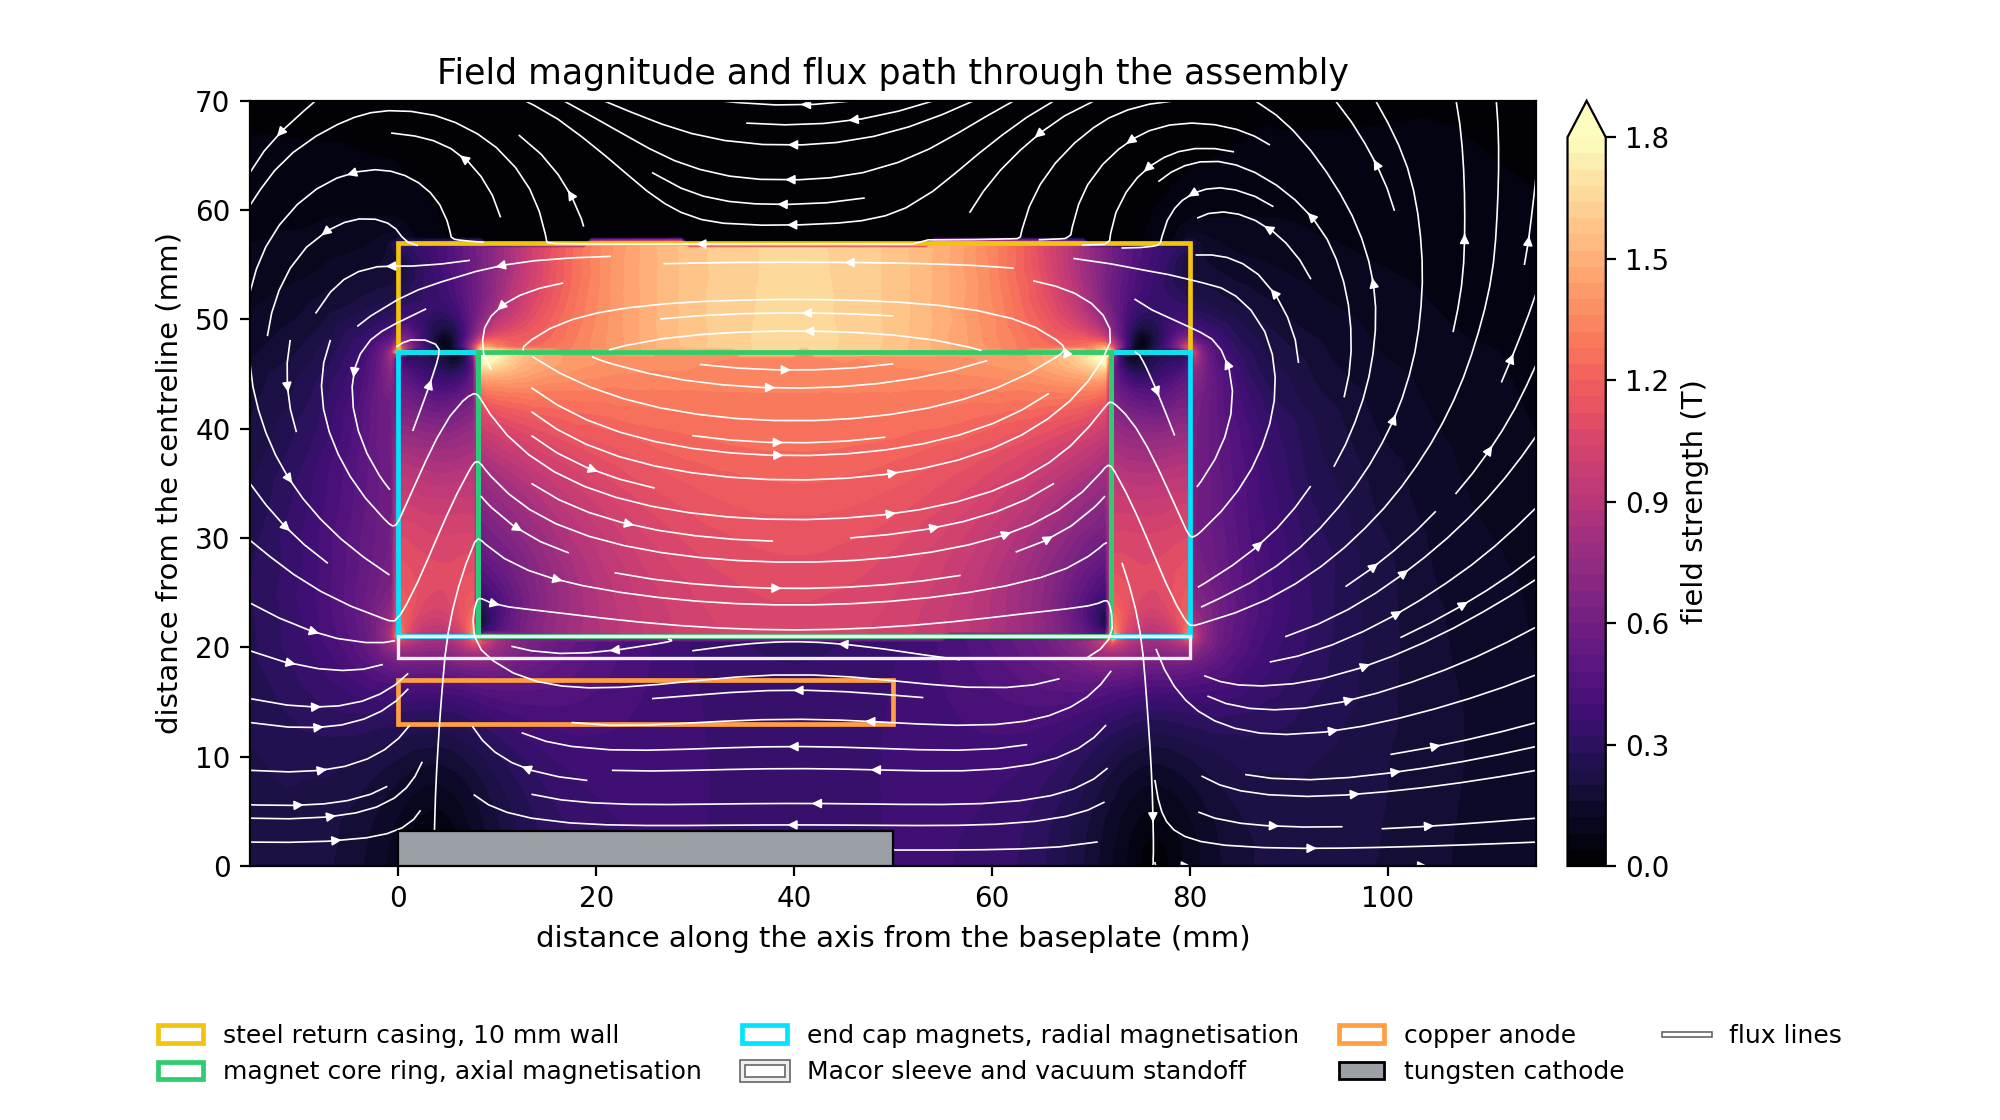
\includegraphics[width=0.72\textwidth]{fig_02_field_map.png}
    \caption{Flux leaves the core ring, runs axially along the steel casing,
    re-enters through the end caps and crosses the bore. That crossing is the
    field the discharge sees, and it is the reason the end caps matter so much:
    without them a magnet tube has almost no bore field at all. The full field
    map was exported for three builds; this is the nearest to the recommended
    one and differs only in cap thickness.}
    \label{fig:map}
\end{figure}

\begin{table}[H]
\centering
\caption{Field of the recommended build, on the axis. Hot figures are the cold
solution scaled by the remanence coefficient at the solved magnet temperature;
that scaling is checked against solved hot cases in Section~\ref{sec:verif}.}
\label{tab:field}
\begin{tabular}{lrr}
\toprule
\textbf{Quantity} & \textbf{Cold, 20~\degC} & \textbf{Hot, 72~\degC} \\
\midrule
$|B_z|$ at the cathode tip, $z = 50$~mm      & 0.669~T & 0.631~T \\
Mean over the channel, $z = 20$ to 50~mm     & 0.657~T & 0.619~T \\
Weakest point in the channel                 & 0.534~T & 0.503~T \\
Strongest point, at $z = 37$~mm              & 0.677~T & 0.638~T \\
\midrule
Ripple over the channel                      & \multicolumn{2}{c}{21.9\%} \\
Length held within 10\% of the peak          & \multicolumn{2}{c}{31.5~mm} \\
Peak flux density in the steel casing        & \multicolumn{2}{c}{1.58~T} \\
\bottomrule
\end{tabular}
\end{table}

Three things follow.

\textbf{The field requirement is met with margin.} Every point in the 30~mm
discharge channel is above 0.50~T hot, against a 0.40~T floor. The thruster
does not merely scrape the requirement at one probe point.

\textbf{The iron is not saturated.} The peak flux density in the casing away
from the magnetisation corners is 1.58~T against a saturation knee near 2.1~T,
so the return path works in its linear region and the field is set by the
geometry rather than by the steel grade or its temperature. The raw maximum
over the whole casing reads 2.51~T, but that is a mathematical singularity at
the four lines where a radially magnetised cap meets an axially magnetised core
against the casing bore. It does not converge under mesh refinement: measured
2.44~T at a 1.5~mm element and 2.97~T at 0.25~mm, still climbing. Real sintered
tiles have a finite transition region and no such line exists, so the
corner-excluded figure is the one that answers the question, and it is stable
to four figures across a fourfold mesh refinement.

\textbf{The uniform region is 31.5~mm, and the requirement is 40 to 70~mm.}
This is the one requirement the recommended build does not meet.
Section~\ref{sec:decision} deals with it, because the fix is cheap and it has to
be decided before the tiles are made.

\subsection{Verification}
\label{sec:verif}
Figure~\ref{fig:twocode} shows the cross-code benchmark between independent
COMSOL and FEMM implementations. The models were constructed independently in
two distinct solvers using identical baseline geometry and material definitions.

\begin{figure}[H]
    \centering
    
\includegraphics[width=\textwidth]{fig_03_two_code_agreement.png}
    \caption{Cross-code verification: FEMM 4.2 against COMSOL 6.4 on the baseline
    magnet stack. They agree to better than half a percent through the channel.
    This serves as a benchmark test ensuring solver fidelity before parametric
    sweeps are executed.}
    \label{fig:twocode}
\end{figure}

\begin{table}[H]
\centering
\caption{The four checks the field results rest on.}
\label{tab:checks}
\begin{tabular}{p{4.2cm}p{6.2cm}l}
\toprule
\textbf{Check} & \textbf{What was done} & \textbf{Result} \\
\midrule
Two independent codes &
FEMM and COMSOL on identical geometry, models built separately &
0.359~T against 0.361~T \\
End cap polarity &
The same stack solved with the caps reversed, as an enforced ratio rather than
an absolute &
factor of 5.0 \\
Remanence scaling &
The hot field scaled from the cold solve, against a uniform temperature sweep
at 60, 100, 140 and 180~\degC &
0.3\% worst case \\
Scaling against a coupled solve &
The same scaling against the thirteen cases solved with both physics together
in the same temperature band &
0.1\% high to 1.4\% low \\
Iron saturation &
Peak flux with a 1~mm skin around the magnetisation corners excluded, across a
fourfold mesh refinement &
stable to four figures \\
\bottomrule
\end{tabular}
\end{table}

The remanence check matters because every hot field in this note is a cold
solve scaled by $1 + \alpha_{Br}\,\Delta T$ with $\alpha_{Br} = -0.11$\% per
kelvin, using the \emph{peak} magnet temperature. Two things have to hold for
that, and they are separate.

The field has to be linear in remanence. It is: over the 52~K rise this design
sees, scaling the cold solve reproduces the separately solved uniform
temperature cases to 0.03\%.

And the peak has to stand in for a stack that is not isothermal. This one runs
from 60~\degC{} in the front cap ring to 72~\degC{} in the rear, and scaling by
the hottest point treats all of it as the hottest point. Measured against the
thirteen cases that were solved with both physics coupled, in the same
temperature band, scaling by the peak lands between 0.1\% high and 1.4\% low,
and low in twelve of the thirteen. \textbf{So 0.631~T is a slightly
conservative figure rather than an optimistic one}, and a coupled solve of this
exact build would be expected to return between 0.631 and 0.640~T.

\subsection{Demagnetisation}
The magnets sit in their own reversed field, so the working point has to be
checked against intrinsic coercivity rather than assumed safe.
Figure~\ref{fig:demag} is that check.

\begin{figure}[H]
    \centering
    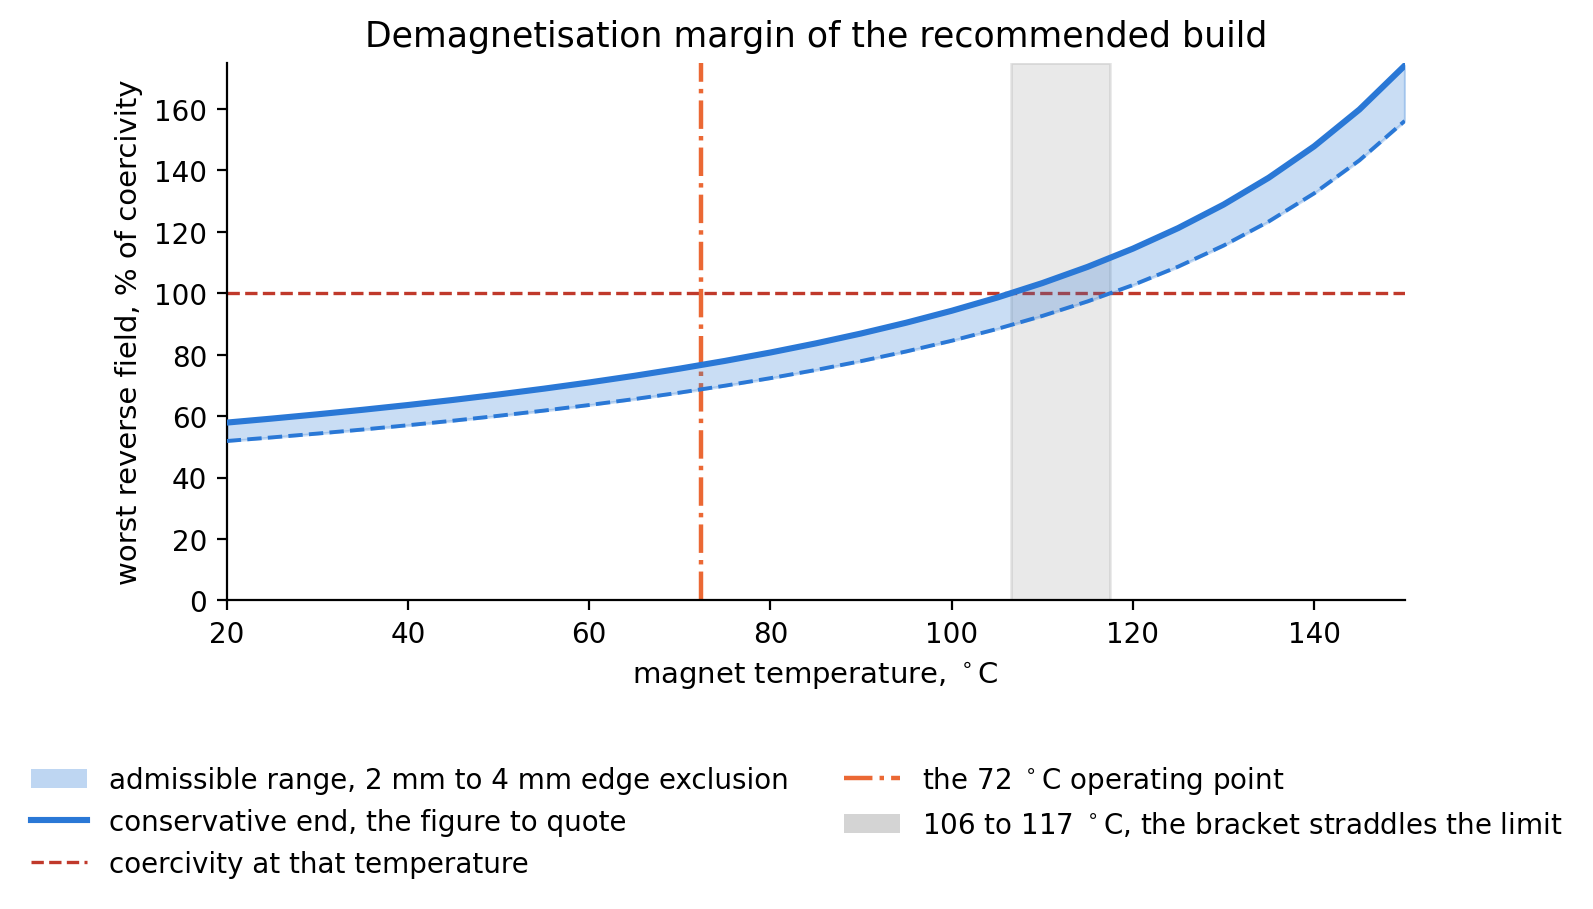
\includegraphics[width=\textwidth]{fig_04_demag_margin.png}
    \caption{The worst reverse field anywhere in the magnet body, as a
    percentage of the coercivity at that temperature. At the 72~\degC{}
    operating point the conservative reading is 77\% and the wider one 69\%, so
    the margin is at least 23\% and no part of the magnet body is past
    coercivity. The demagnetised volume fraction is zero.}
    \label{fig:demag}
\end{figure}

The reverse field is singular at eight edges, where the cap and core
magnetisations meet and where the magnetisation stops at the ends of the stack.
Masking a skin around those edges does not converge: a sweep from 0.5 to 10~mm
falls monotonically the whole way, because unlike the iron singularity, which
sits on isolated points, the magnet reverse field is largest along an extended
region of the bore. So the pair of mask widths is a \emph{bracket}, not a
convergence test.

It is still enough to answer the question, for two reasons. Every mask below
2~mm returns a field above the physical self-demagnetisation bound $B_r/\mu_0$
and is therefore still reading the singularity, which puts a floor on the
admissible range. And widening the mask only ever reduces the magnitude, which
makes the narrow end the conservative one. \textbf{Quote bounds, not values:}
``at least a 23\% margin at the operating point'' is safe and ``a 23\%
margin'' is not. Between about 106 and 117~\degC{} the two widths straddle the
limit and nothing should be quoted there at all. That is well clear of the
72~\degC{} the design runs at.

% =====================================================================
\section{Thermal Design}
\label{sec:thermal}
% =====================================================================

\subsection{Thermal Management Requirements and Architecture Trade}
For continuous operation, relying on transient thermal mass to absorb the 500~W
arc deposition is unfeasible. Figure~\ref{fig:concepts} evaluates four rear interface
architectures side by side under continuous 500~W load.

\begin{figure}[H]
    \centering
    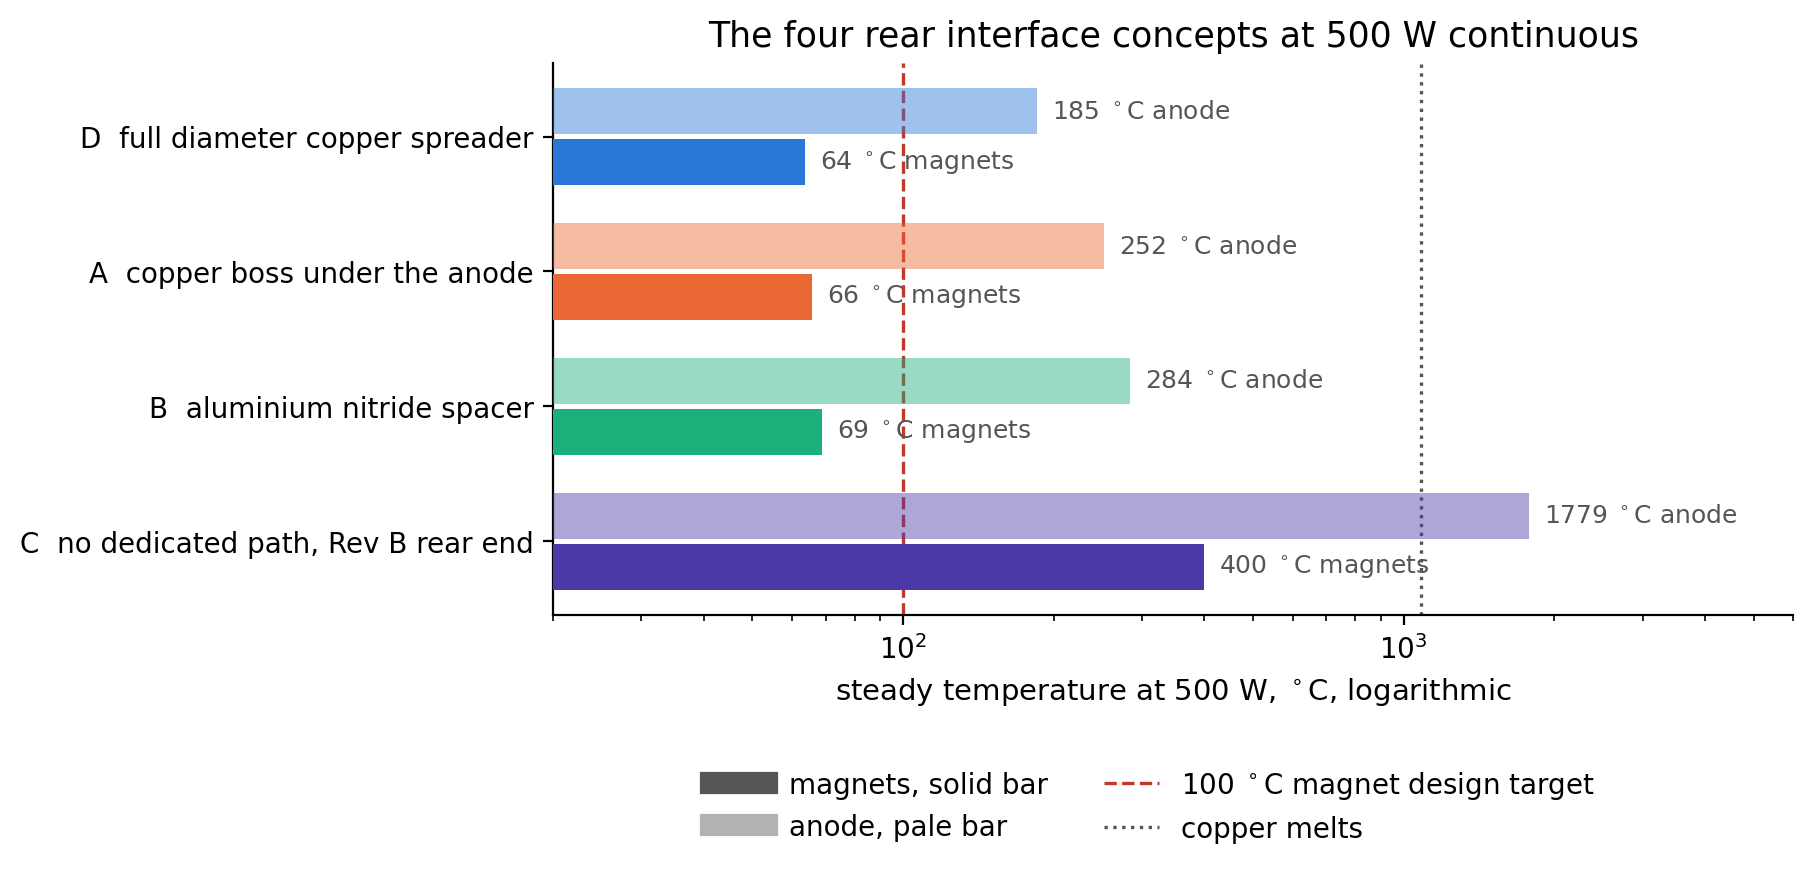
\includegraphics[width=\textwidth]{fig_05_rear_concepts.png}
    \caption{Evaluation of four rear interface concepts at 500~W continuous thermal
    load on a logarithmic scale. Concept~C represents an uncooled baseline without
    axial heat extraction: the anode reaches 1779~\degC{} (exceeding copper's melting
    point) and magnets reach 400~\degC{} (exceeding Curie temperature). Concepts A,
    B, and D all successfully maintain the magnets between 64 and 69~\degC.}
    \label{fig:concepts}
\end{figure}

The four are compared on one common radial build, with a 4~mm anode wall and a
2~mm break, so that the only thing that differs between them is the rear end.
The recommended build has a thinner anode and a narrower break and therefore
runs hotter than the Concept~D bar shown here; its own temperatures are in
Table~\ref{tab:temps}.

Concepts A, B and C are the three the brief asked for. \textbf{D was added},
and the reason is arithmetic worth keeping. Concept~A hands the heat off over
the anode footprint only, an annulus of $1.1 \times 10^{-3}$~m$^2$. Spread the
same heat over the full 114~mm rear face, $1.0 \times 10^{-2}$~m$^2$, and the
same interface coefficient is nine times better. That is the argument, and it
costs one copper disc.

The run says the argument is directionally right and quantitatively overstated,
and that is worth knowing. Concept~A does not fail: it puts the magnets at
66~\degC{} and the anode at 252~\degC, against 64 and 185 for Concept~D. The
small footprint costs 67~K on the anode, not the hundreds of kelvin the area
ratio implies. What rescues it is the isolation plate, which is aluminium
nitride at 170~W/(m$\cdot$K) running the full diameter, so it spreads the heat
before the cold plate whatever sits above it. \textbf{Concept~D is still the
better build and is the recommended one}, but the margin is 67~K on the anode
rather than a pass and a fail.

The obvious objection to Concept~D is that a copper disc at full diameter sits
directly behind the magnets, which is exactly the leak path the brief warns
about. But the disc runs between 63 and 83~\degC, not 400. The magnets sitting
on a 10~mm Macor shelf above it do not care. \textbf{The conflict between getting the
heat out and keeping it off the magnets is far weaker than it looks, as long as
the spreader runs cold.}

\subsection{What the recommended build actually does}

\begin{figure}[H]
    \centering
    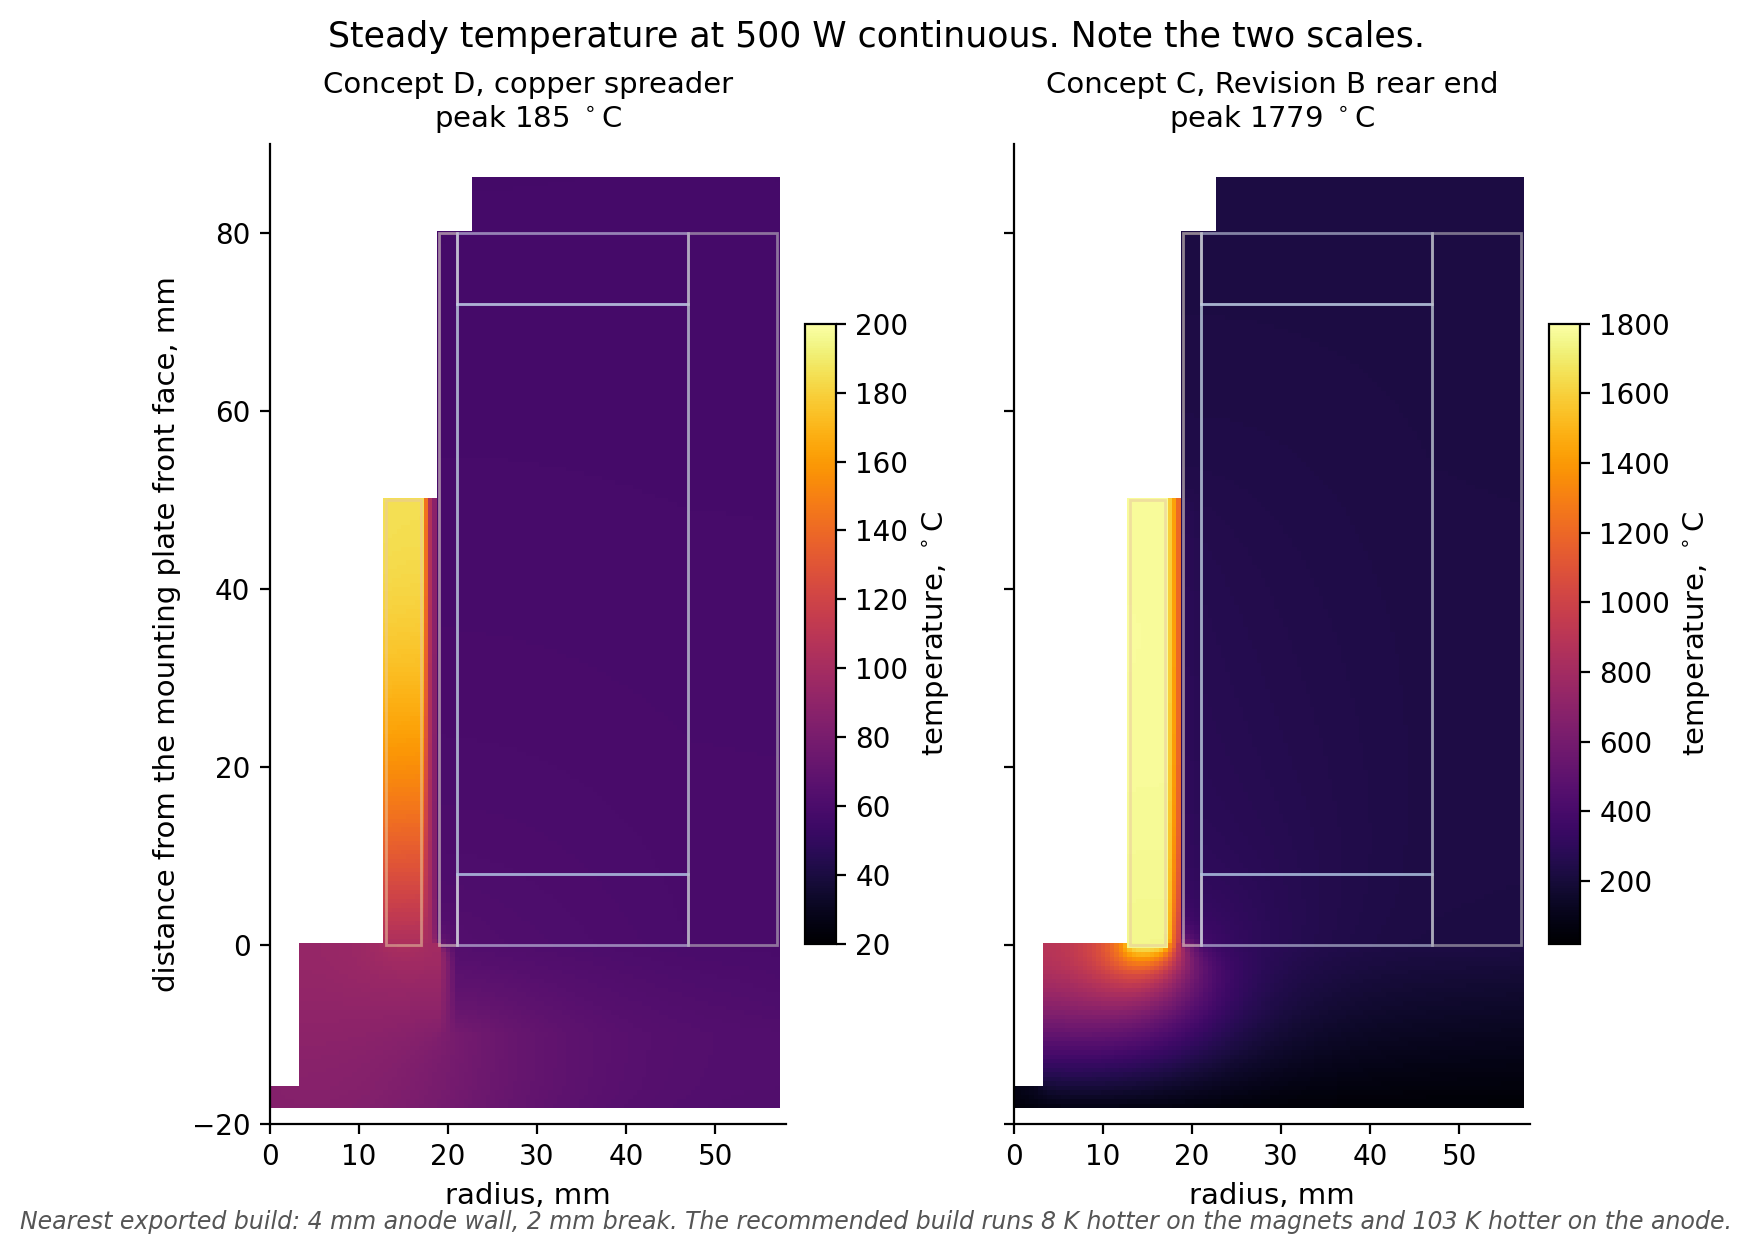
\includegraphics[width=\textwidth]{fig_06_temperature_field.png}
    \caption{Steady-state temperature distribution at 500~W continuous: settled
    Concept~D architecture compared to the uncooled baseline configuration. Note the
    distinct colour scales reflecting a tenfold thermal divergence. In Concept~D, heat
    conducts axially backwards through the anode and dissipates across the rear stack,
    keeping all components outboard of the thermal break near 60~\degC.}
    \label{fig:tempfield}
\end{figure}

\begin{table}[H]
\centering
\caption{Steady temperatures of the recommended build at 500~W continuous, with
the rear interface at 1000~W/(m$^2\cdot$K).}
\label{tab:temps}
\begin{tabular}{lrr}
\toprule
\textbf{Location} & \textbf{Peak, \degC} & \textbf{Minimum, \degC} \\
\midrule
Anode, at the exit plane          & 288 & 110 \\
Radiation shield                  & 135 & 106 \\
Standoff sleeve                   & 106 &  59 \\
\textbf{Magnets, rear cap ring}   & \textbf{72} & \textbf{61} \\
Magnets, core rings               &  66 &  60 \\
Magnets, front cap ring           &  60 &  60 \\
Iron casing                       &  62 &  60 \\
Macor magnet shelf                &  83 &  61 \\
Isolation plate                   &  89 &  62 \\
Cold plate face                   & \multicolumn{2}{c}{63} \\
\bottomrule
\end{tabular}
\end{table}

\textbf{The magnets peak at 72~\degC{} against a 100~\degC{} design target and a
180~\degC{} rating.} The hottest magnets are in the rear cap ring, nearest the
hand-off, which is why the Macor shelf under them is deliberately not a
conductor.

\begin{figure}[H]
    \centering
    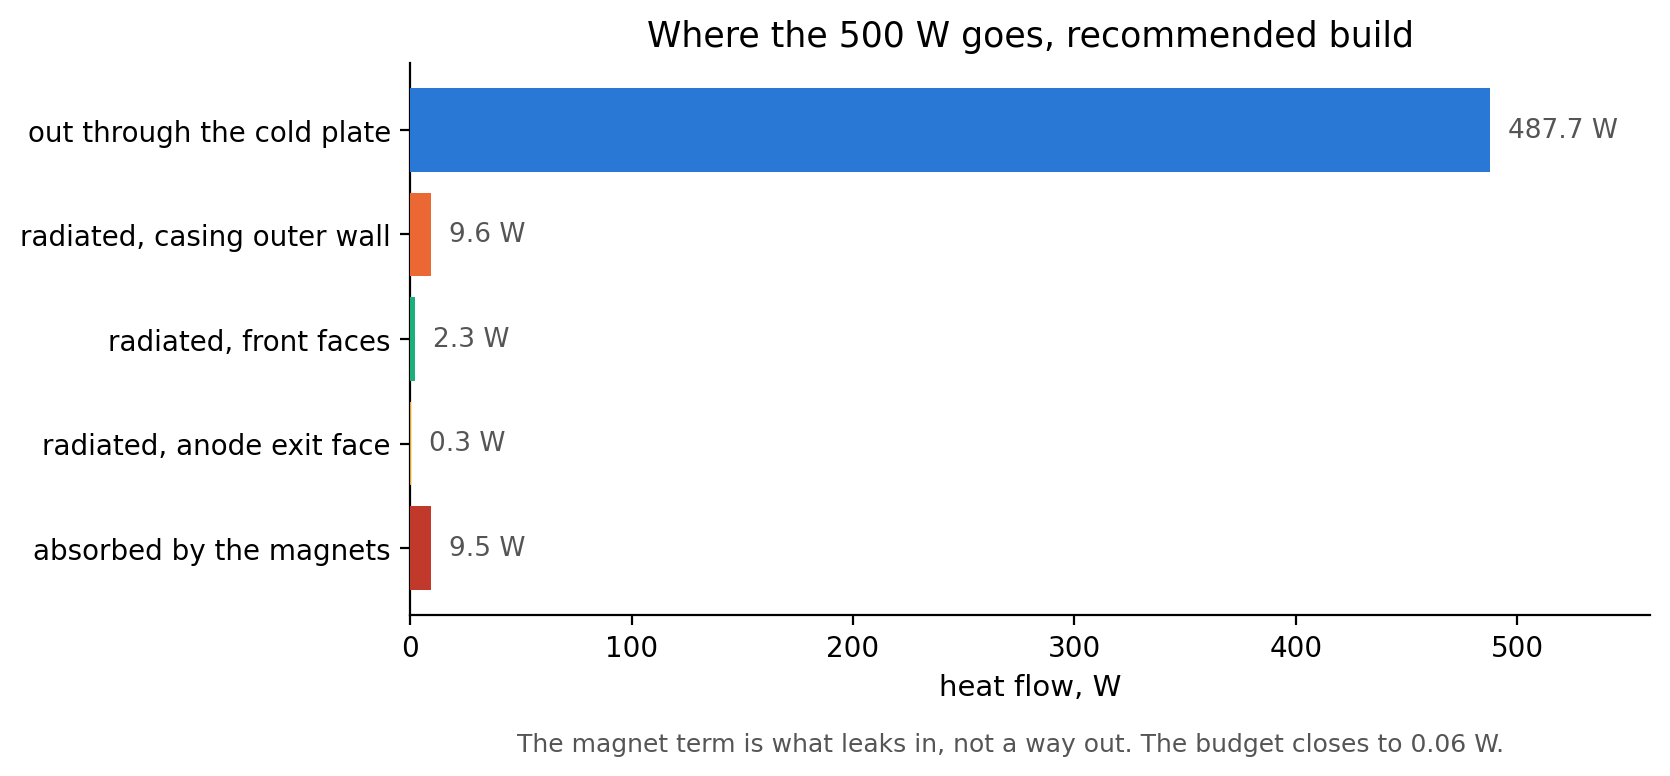
\includegraphics[width=\textwidth]{fig_07_heat_budget.png}
    \caption{Where the 500~W goes in the recommended build. Almost all of it
    leaves through the cold plate; 9.6~W radiates from the casing outer wall,
    and 9.5~W leaks into the magnets. That last term is not a way out, it is
    what gets in. The budget closes to 0.06~W here and to better than a third
    of a watt on every one of the 84 thermal cases, which is the check that the
    model conserves energy.}
    \label{fig:budget}
\end{figure}

\subsection{Why these dimensions, and not thicker ones}
The central design tension is that both thermal levers, a thicker
anode wall and a wider evacuated break, push the magnet bore outwards, and the
bore field of a Halbach stack falls steeply with bore radius.
Figure~\ref{fig:trade} is that trade measured rather than argued.

\begin{figure}[H]
    \centering
    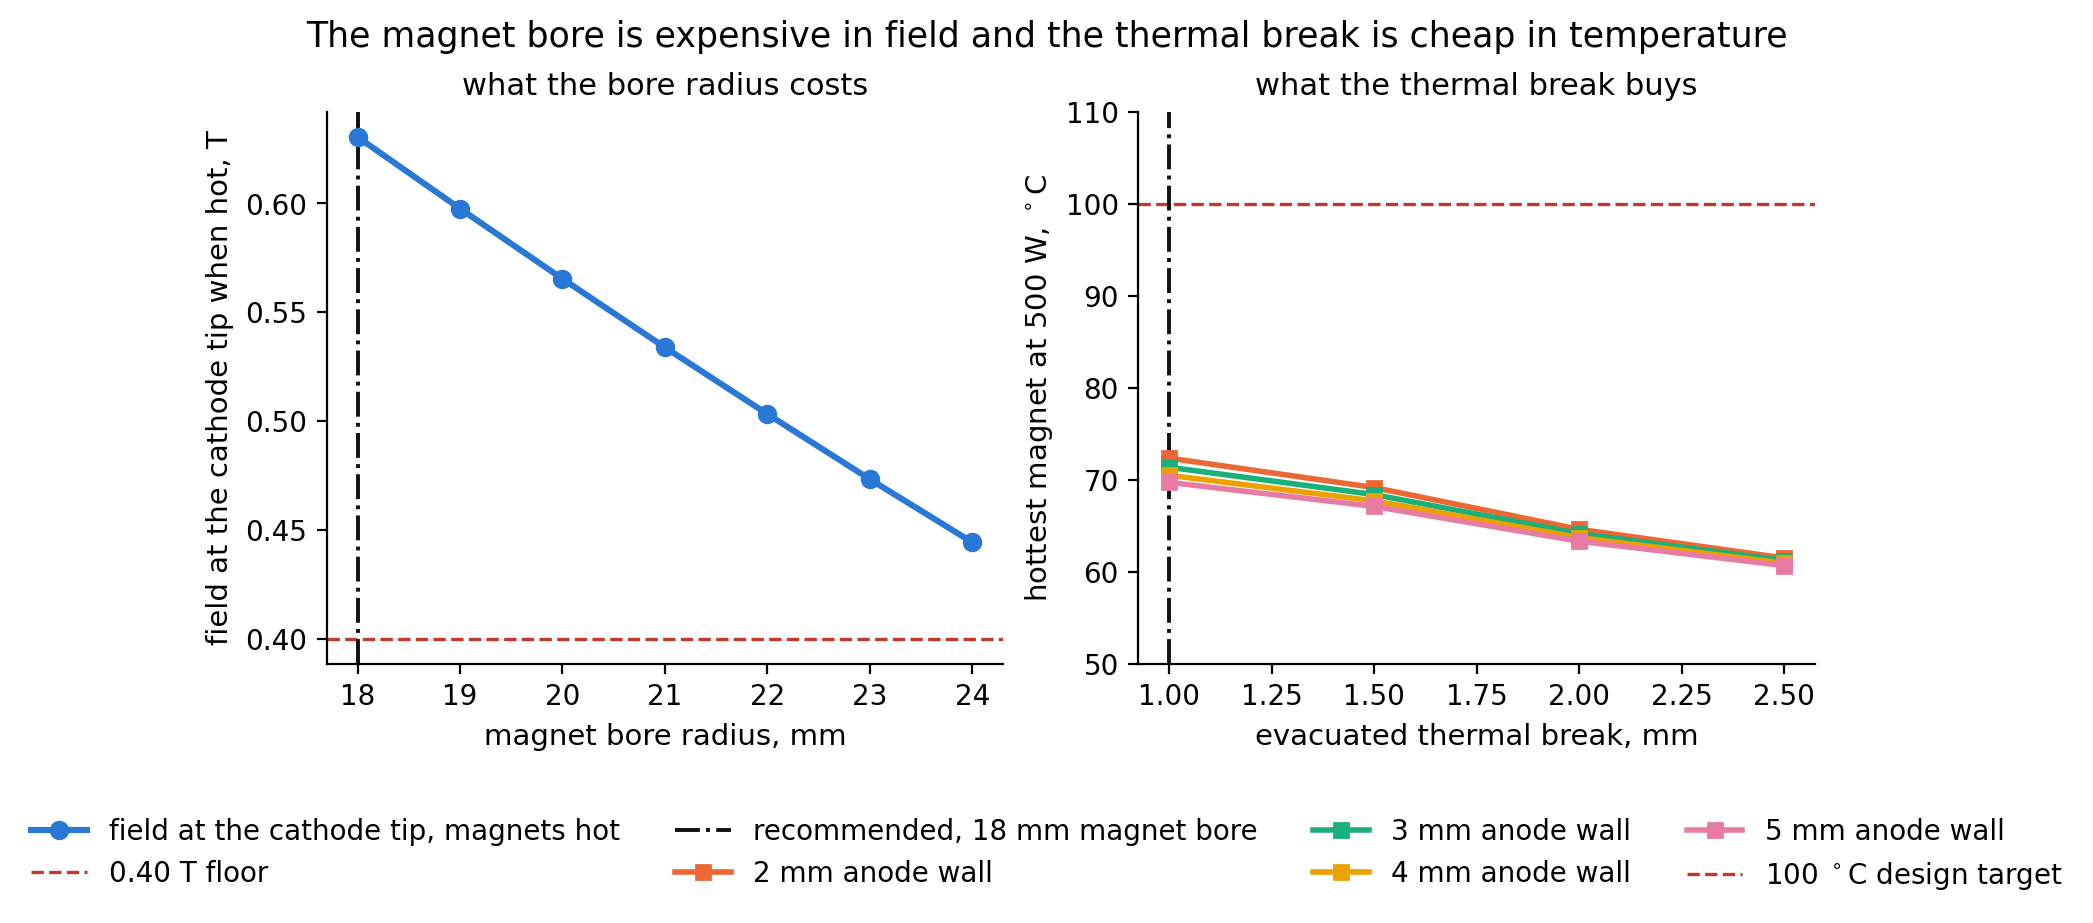
\includegraphics[width=\textwidth]{fig_08_bore_radius_trade.png}
    \caption{Left: field at the cathode tip against magnet bore radius. Every
    millimetre outwards costs about 0.031~T. Right: the hottest magnet against
    the width of the evacuated break, for four anode wall thicknesses. Widening
    the break from 1.0 to 2.5~mm buys 11~K and costs 0.05~T, and the 11~K is
    margin the design does not need.}
    \label{fig:trade}
\end{figure}

\begin{table}[H]
\centering
\caption{Anode wall thickness against the two temperatures it sets, at a 1~mm
break. The wall is the anode's own conduction path to the rear. The field
column is read off the magnet bore radius, because nothing between the bore and
the magnets is magnetic, so a millimetre of copper and a millimetre of vacuum
cost exactly the same field.}
\label{tab:wall}
\begin{tabular}{lrrr}
\toprule
\textbf{Anode wall} & \textbf{Hottest anode, \degC} & \textbf{Hottest magnet, \degC}
& \textbf{Cold field, T} \\
\midrule
\textbf{2~mm} & \textbf{288} & \textbf{72} & \textbf{0.669} \\
3~mm & 220 & 71 & 0.634 \\
4~mm & 185 & 71 & 0.600 \\
5~mm & 163 & 70 & 0.566 \\
\bottomrule
\end{tabular}
\end{table}

The 2~mm wall is chosen because 288~\degC{} is comfortably below the 400~\degC{}
at which copper begins to soften, and because each millimetre of wall costs
0.035~T while buying nothing at all on the magnets. The anode is the only part
that gets hot, and it has 112~K of margin.

The evacuated break is kept at 1~mm for the same reason. It does most of the
work of keeping heat off the magnets: at mid channel the anode outer wall sits
at 244~\degC{} and the sleeve bore at 62~\degC, so 1~mm of vacuum drops 182~K.
Widening it to 2.5~mm buys a further 11~K on the magnets and costs about
0.05~T. The 0.3~mm polished radiation shield
inside it is worth about 1~K and may be deleted without consequence if the
0.35~mm clearance each side proves awkward to build.

\subsection{The requirement this design places on somebody else}
Everything above assumes the external interface at $z = -18$~mm can take the
heat away. It is modelled as a contact coefficient and swept over a factor of
fifty, because nobody knows it yet.

\begin{figure}[H]
    \centering
    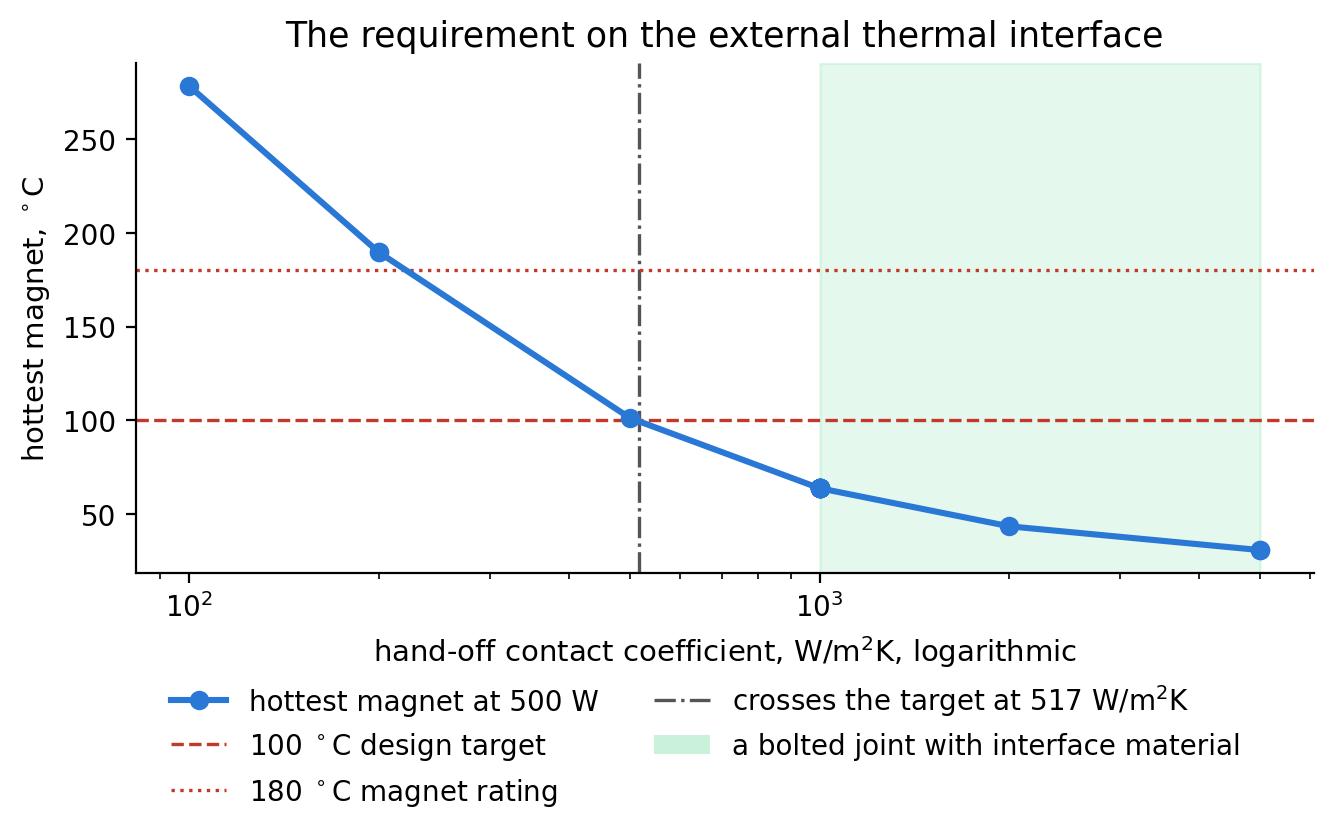
\includegraphics[width=\textwidth]{fig_09_sink_requirement.png}
    \caption{The single number to hand to whoever designs the cold plate. Below
    about 520~W/(m$^2\cdot$K) the magnets pass the 100~\degC{} design target;
    above about 2000 the design has margin to spare. A bolted joint with a
    thermal interface material lands between 1000 and 5000, so the requirement
    is achievable, but it is a requirement and not an assumption.}
    \label{fig:sink}
\end{figure}

\textbf{Specify 1000~W/(m$^2\cdot$K) or better at the hand-off face.} That is
the value every number in Table~\ref{tab:temps} is computed at, and it is a
routine figure for a bolted joint with interface material. The sweep was run on
the 4~mm anode build; the recommended build runs about 9~K hotter on the
magnets, so treat the 520~W/(m$^2\cdot$K) crossing as an absolute floor rather
than a target.

\subsection{If 500 W is wrong}
The nominal design point assumes 500~W of arc power deposited into the anode. For a 1
to 5~kW class thruster the real figure could be several times that, so the sweep
runs to 1500~W.

\begin{figure}[H]
    \centering
    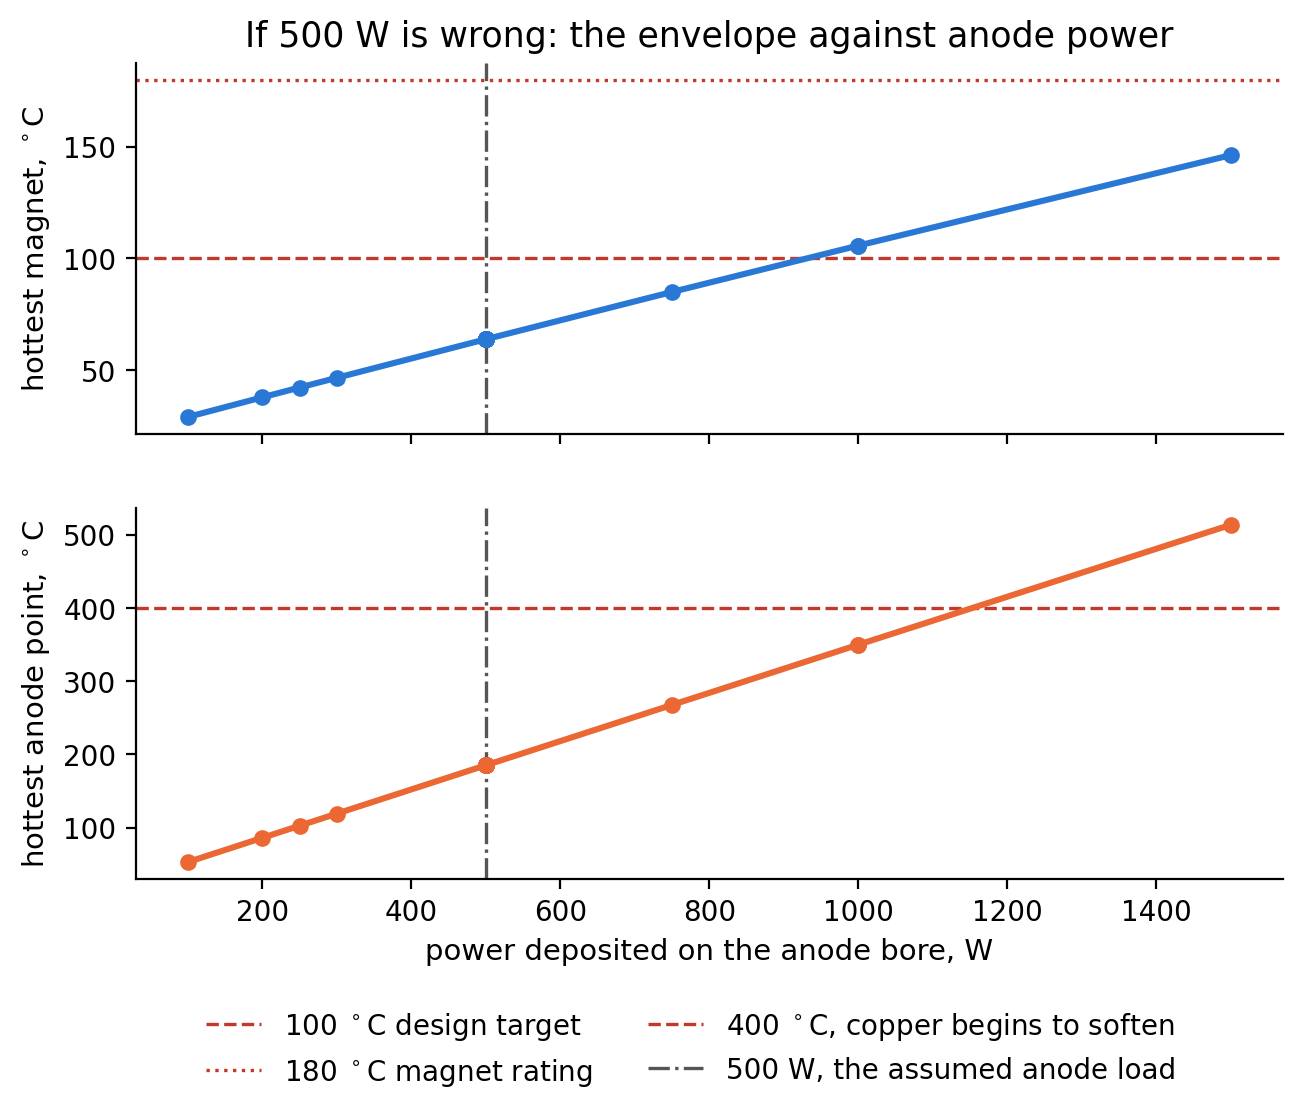
\includegraphics[width=\textwidth]{fig_10_power_envelope.png}
    \caption{Operating envelope against anode power, for the 4~mm anode wall
    the sweep was run on. At the design interface coefficient the magnets stay
    inside the 100~\degC{} target to about 900~W and inside the 180~\degC{}
    rating well beyond 1500~W, and the anode reaches 400~\degC{} near 1150~W.
    The recommended 2~mm wall runs hotter: scaling its 500~W result gives
    100~\degC{} magnets near 760~W and a 400~\degC{} anode near 700~W.}
    \label{fig:power}
\end{figure}

\subsection{What the thermal model does and does not include}
Stated plainly, because a reader who does not know these will over-trust the
numbers.

\begin{itemize}[itemsep=3pt]
  \item \textbf{The evacuated break is modelled as a conducting solid} whose
        conductivity is the linearised radiation analogy
        $k = 4\sigma F t T^3$, which is exact for grey diffuse exchange between
        long concentric cylinders. The shield splits it into two such exchanges
        in series. One case was checked against a true surface-to-surface
        solve: 62.1~\degC{} against 63.7~\degC{} on magnet peak temperature, a
        difference of 2.6\%, with 0.99~W crossing the voided gap, which is also
        the proof that the radiation features were live rather than silently
        doing nothing.
  \item \textbf{Joints inside the assembly are perfect.} No contact resistance
        between the anode and the mounting plate or between the rear layers.
        The one interface that is not assumed perfect is the hand-off face
        itself, which is why it is swept.
  \item \textbf{The cathode is not in the thermal model.} It carries its own
        heat load and its own conduction path to the rear, and putting it in
        properly needs a plasma sheath boundary condition that does not exist
        yet. This is a known omission and it makes the results slightly
        optimistic.
  \item \textbf{The magnet stack is a smeared ring, not 40 discrete tiles.}
        Circumferential ripple from the eight-tile rings is not captured by an
        axisymmetric model. 3D finite-element evaluations confirm that this azimuthal modulation has a
        negligible effect on the centreline.
\end{itemize}

% =====================================================================
\section{Would the Thruster Actually Work}
\label{sec:system}
% =====================================================================

A field of the right strength in the right place is necessary and not
sufficient. This section is the evidence that the rest of the machine follows.

\subsection{The magnetic nozzle}
Downstream of the cathode tip the field is no longer confining the discharge,
it is steering the exhaust.

\begin{figure}[H]
    \centering
    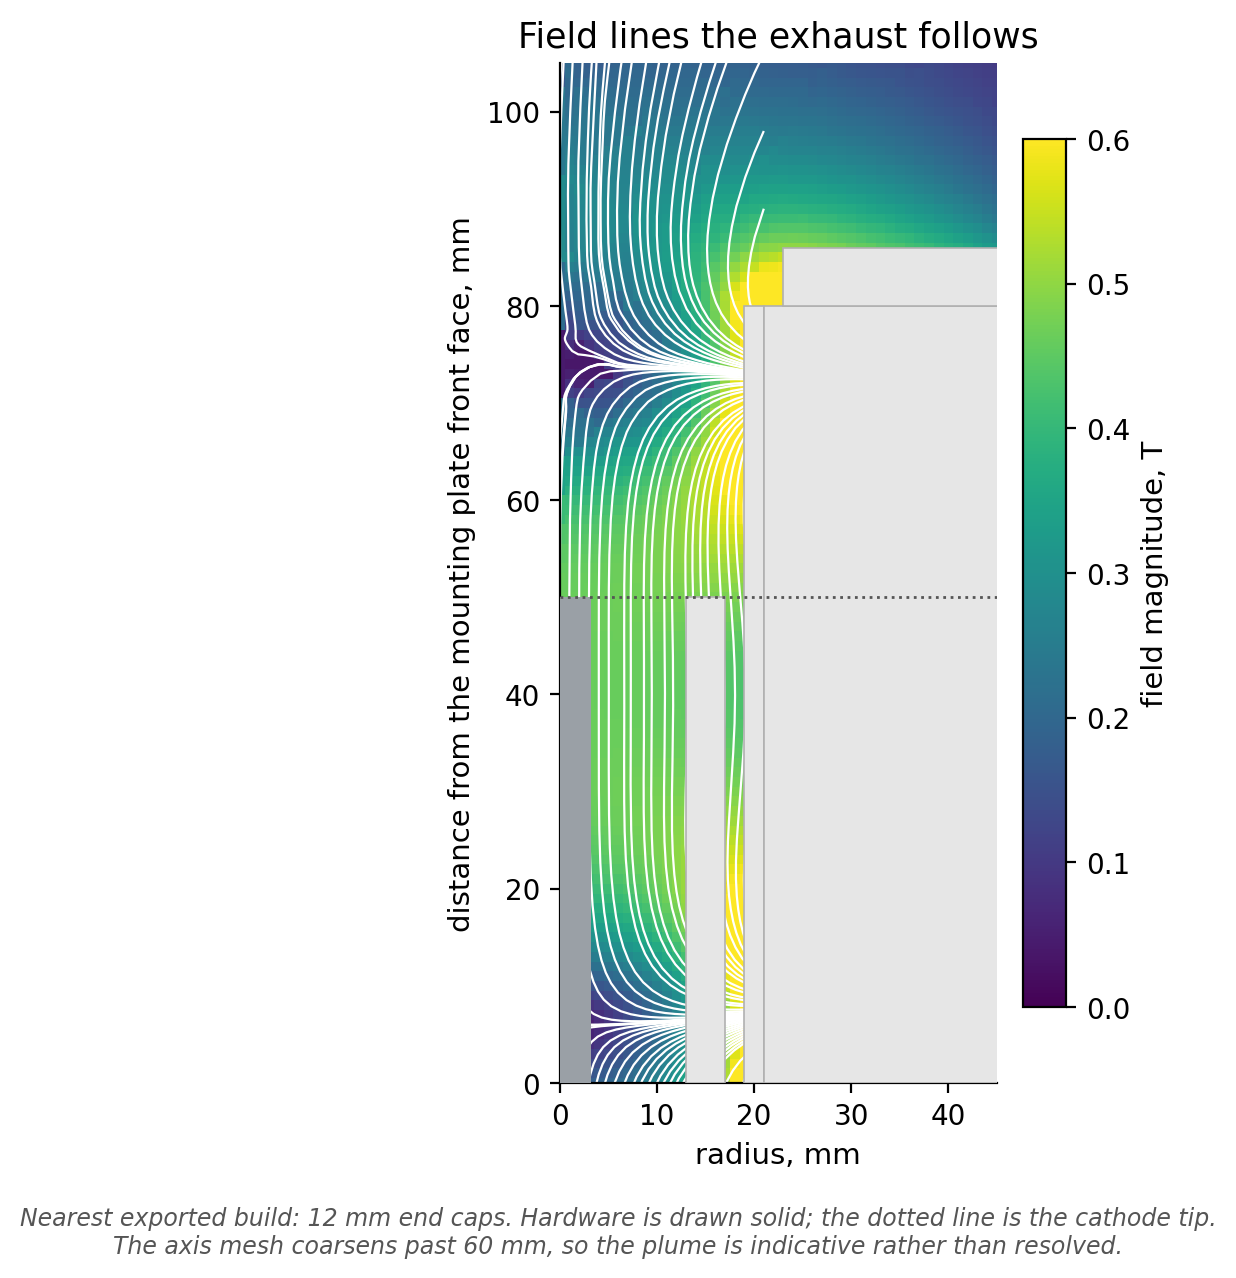
\includegraphics[width=0.70\textwidth]{fig_11_magnetic_nozzle.png}
    \caption{Field lines the exhaust follows. Plasma is tied to field lines, so
    where the lines go the exhaust goes. They converge through the channel,
    pass the cathode tip, and then diverge into the plume. No divergence angle
    is quoted: tracing a line through the field reversal near $z = 70$~mm is
    ill conditioned and the mesh out there is coarse.}
    \label{fig:nozzle}
\end{figure}

\textbf{On the centreline the field passes through zero twice}, at $z = 8$~mm
and $z = 70$~mm. This is intrinsic to a permanent magnet ring and cannot be
designed out: inside the bore the field opposes the magnetisation and outside
it aligns with it, so a reversal near each end face is unavoidable. Parametric investigations evaluated six end configurations, including substituting
either cap with soft iron and incorporating an iron snout; none eliminates the nulls,
they merely translate their axial positions.

What can be said instead turns on a distinction worth being careful about:
\emph{the centreline is not the discharge}. The cathode is a 6.35~mm tungsten
rod running the full length of the anode, so the plasma occupies an annulus
from $r = 3.175$~mm out to the anode bore at $r = 13$~mm. The axis inside that
rod is solid metal. That places the upstream null \emph{inside the cathode
rod}, where no plasma reaches it, and the downstream null 20~mm past the
cathode tip, out in the plume and clear of all hardware. In the annulus the
plasma actually occupies, the weakest field anywhere is 0.056~T and 98\% of the
annulus is above 0.1~T. Those two off-axis figures were measured on the 12~mm
cap build, which is the nearest one for which the bore was mapped off the axis;
they are indicative for the recommended build rather than solved for it.

\subsection{Where the current flows and what it does}

\begin{figure}[H]
    \centering
    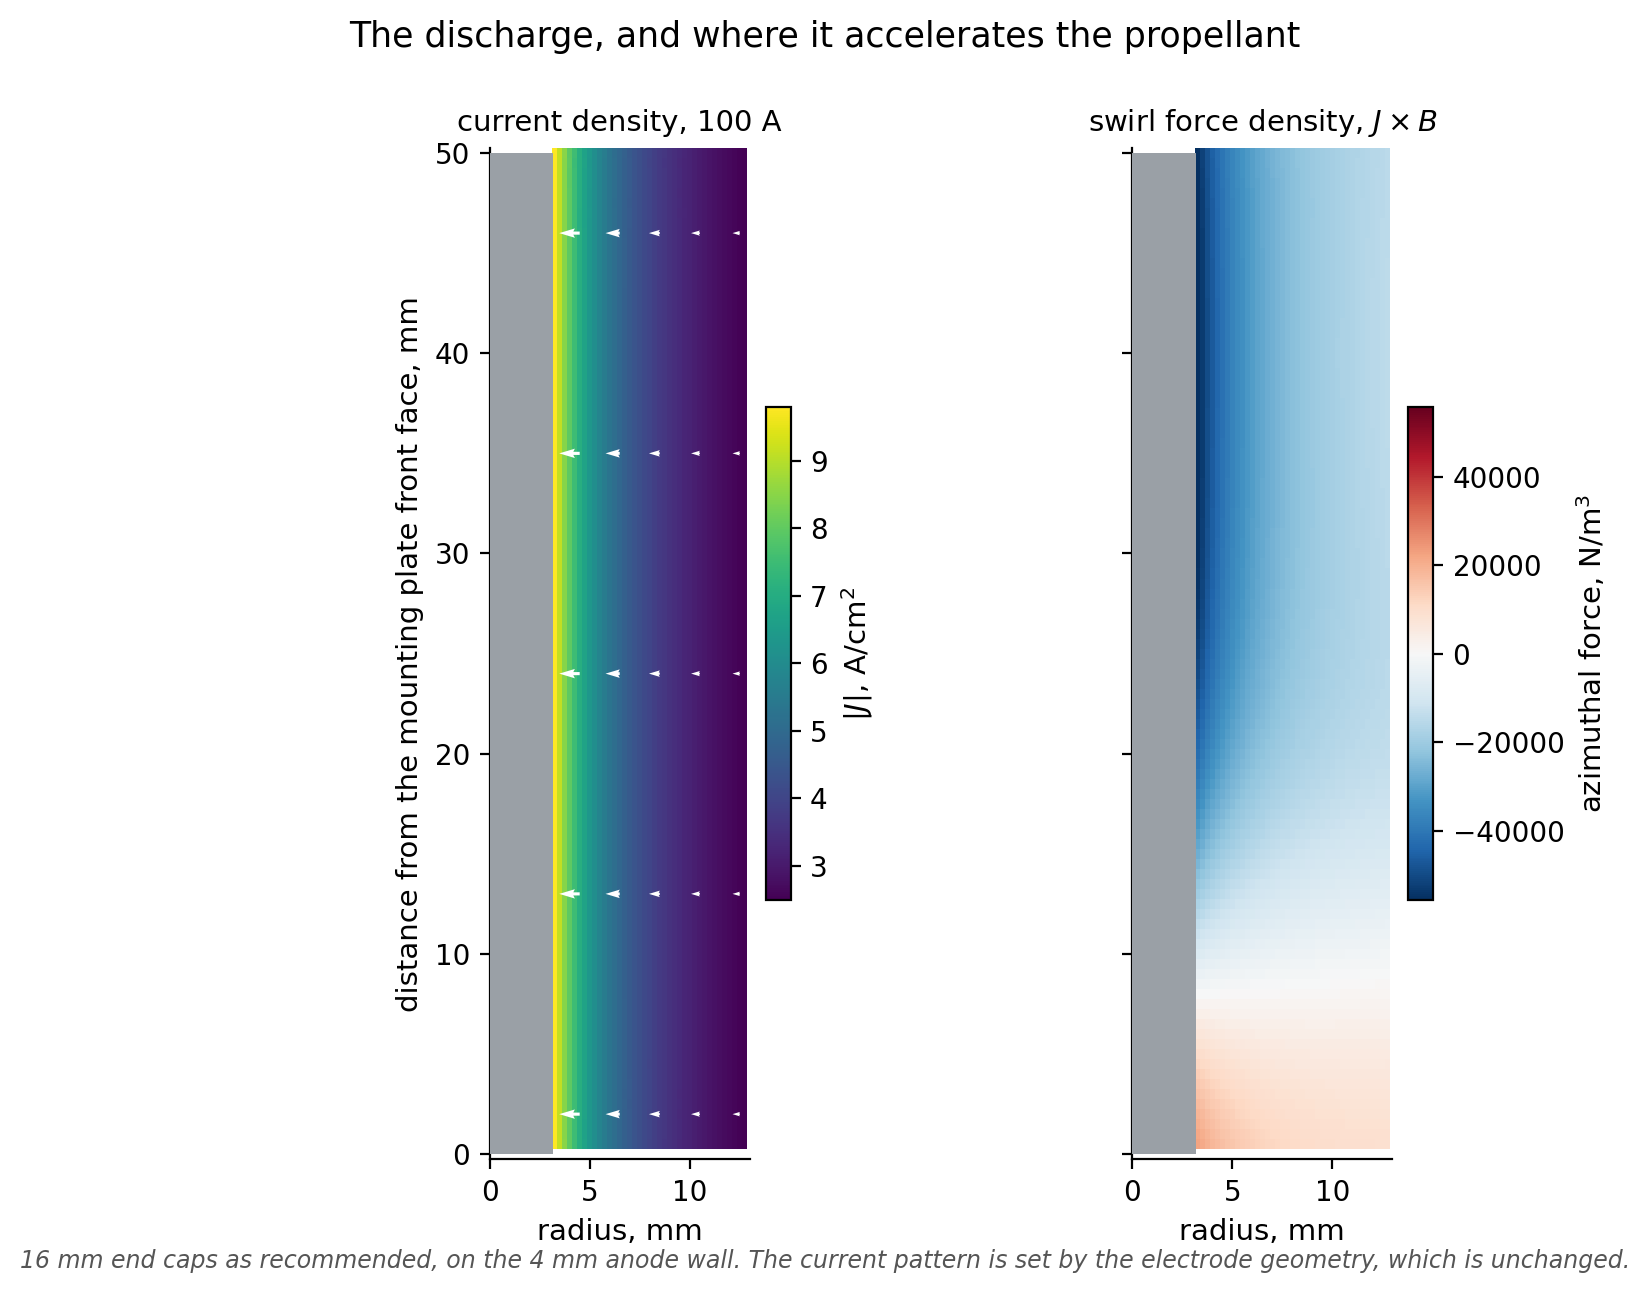
\includegraphics[width=\textwidth]{fig_12_current_and_swirl.png}
    \caption{The argon column modelled as a uniform conductor between the real
    electrode surfaces. Current runs almost straight out from the cathode to
    the anode wall. Crossed with the applied field it gives an azimuthal force
    that spins the propellant up, strongest over the downstream two thirds of
    the channel, and that swirl is recovered as thrust in the nozzle.}
    \label{fig:current}
\end{figure}

\textbf{This is not a plasma simulation.} There is no ionisation, no separate
electron and ion temperatures, no sheath physics at the electrodes and no flow.
For a medium of uniform conductivity the \emph{shape} of the current pattern is
set by the electrode geometry and not by the conductivity value, which is what
makes it worth solving without a plasma code, and that shape is a large
improvement on assuming the current spreads uniformly.

Two results come out of it that are worth stating. At 100~A the field the
discharge makes is \textbf{0.33\% of the field the magnets make}, so the
magnetostatics and the discharge can legitimately be solved in sequence rather
than simultaneously; that ratio is computed rather than assumed. And the
self-field thrust, the Maecker term that a self-field MPD thruster runs on, is
2.2~mN. \textbf{This thruster is applied-field dominated by two orders of
magnitude}, which is the whole premise of the programme and is now a number
rather than an assertion.

\begin{figure}[H]
    \centering
    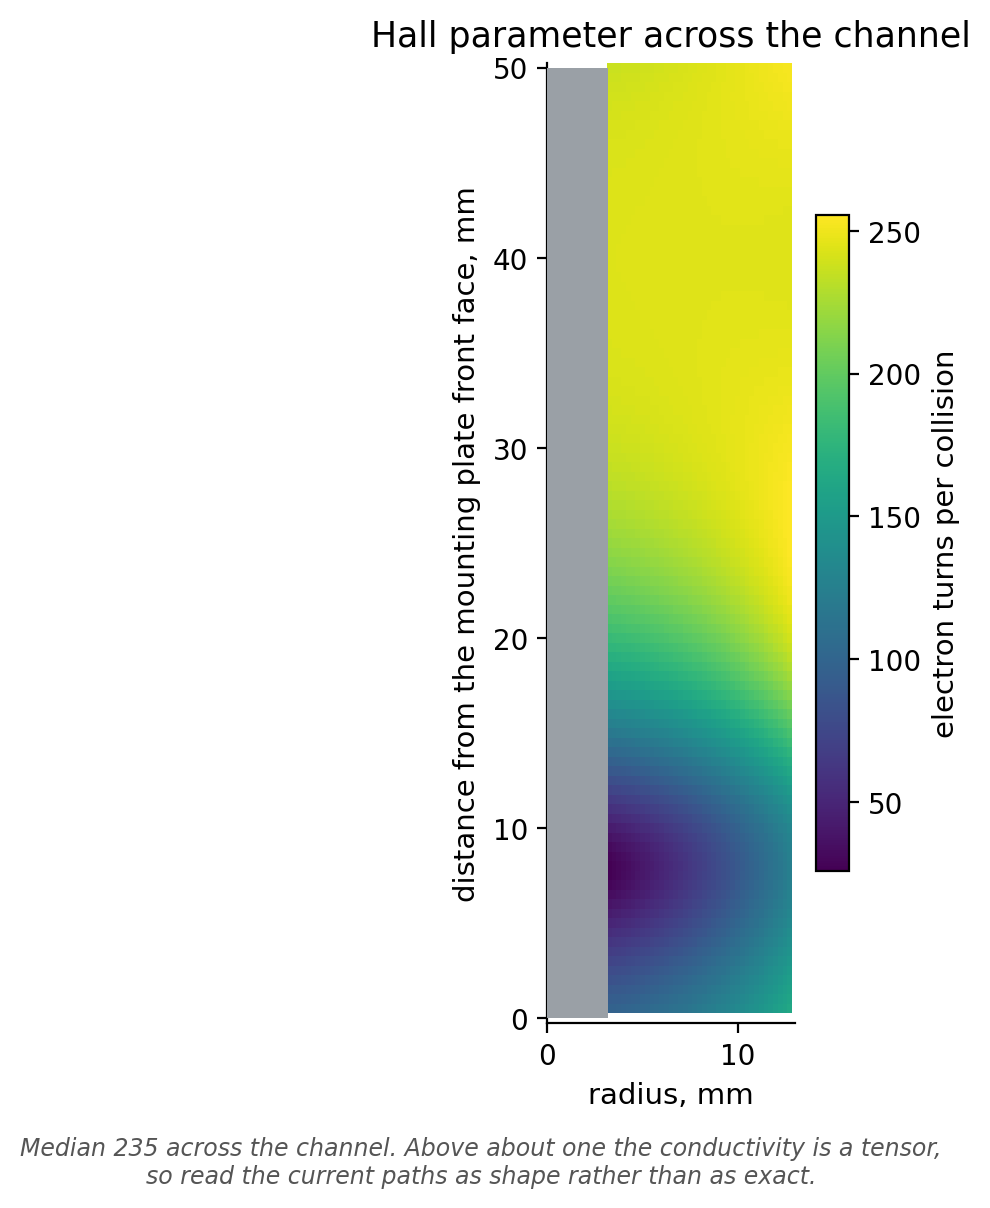
\includegraphics[width=0.55\textwidth]{fig_13_hall_parameter.png}
    \caption{The Hall parameter, the number of turns an electron makes around a
    field line between collisions. The channel median is 235. This is the
    honest limitation of the previous figure: above about one the real
    conductivity is a tensor rather than a scalar, so the current paths should
    be read as indicative of shape rather than as exact.}
    \label{fig:hall}
\end{figure}

\subsection{Predicted thrust}
Thrust is predicted by interpolating measured hardware rather than by
simulating a plasma, because until this thruster exists and is fired there is
nothing to validate a plasma model against. The AFMPDT database holds 2672
published runs, of which 667 are argon. Applied-field thrust scales as the
product of discharge current, applied field at the cathode tip and anode
radius; fitting that scaling to the 62 argon runs nearest this operating point
and evaluating it for this geometry gives:

\begin{itemize}[itemsep=2pt]
  \item \textbf{Best estimate: 186~mN} at 100~A with 0.631~T at the cathode tip.
  \item \textbf{Likely range: 93 to 226~mN}, from the interquartile spread of
        the fit residuals.
\end{itemize}

Two caveats, both real. The fitted runs cover 0.10 to 0.40~T, so 0.63~T is an
extrapolation of about 58\% beyond the data, and the scaling is linear in field
so the extrapolation is at least well behaved. And the spread is wide because
the measured data is scattered, which is a feature of AF-MPD performance rather
than a shortcoming of the fit. For contrast, an unoptimised baseline geometry yields
106~mN under identical evaluation.

\subsection{The feasible set, and the 0.70 T goal}

\begin{figure}[H]
    \centering
    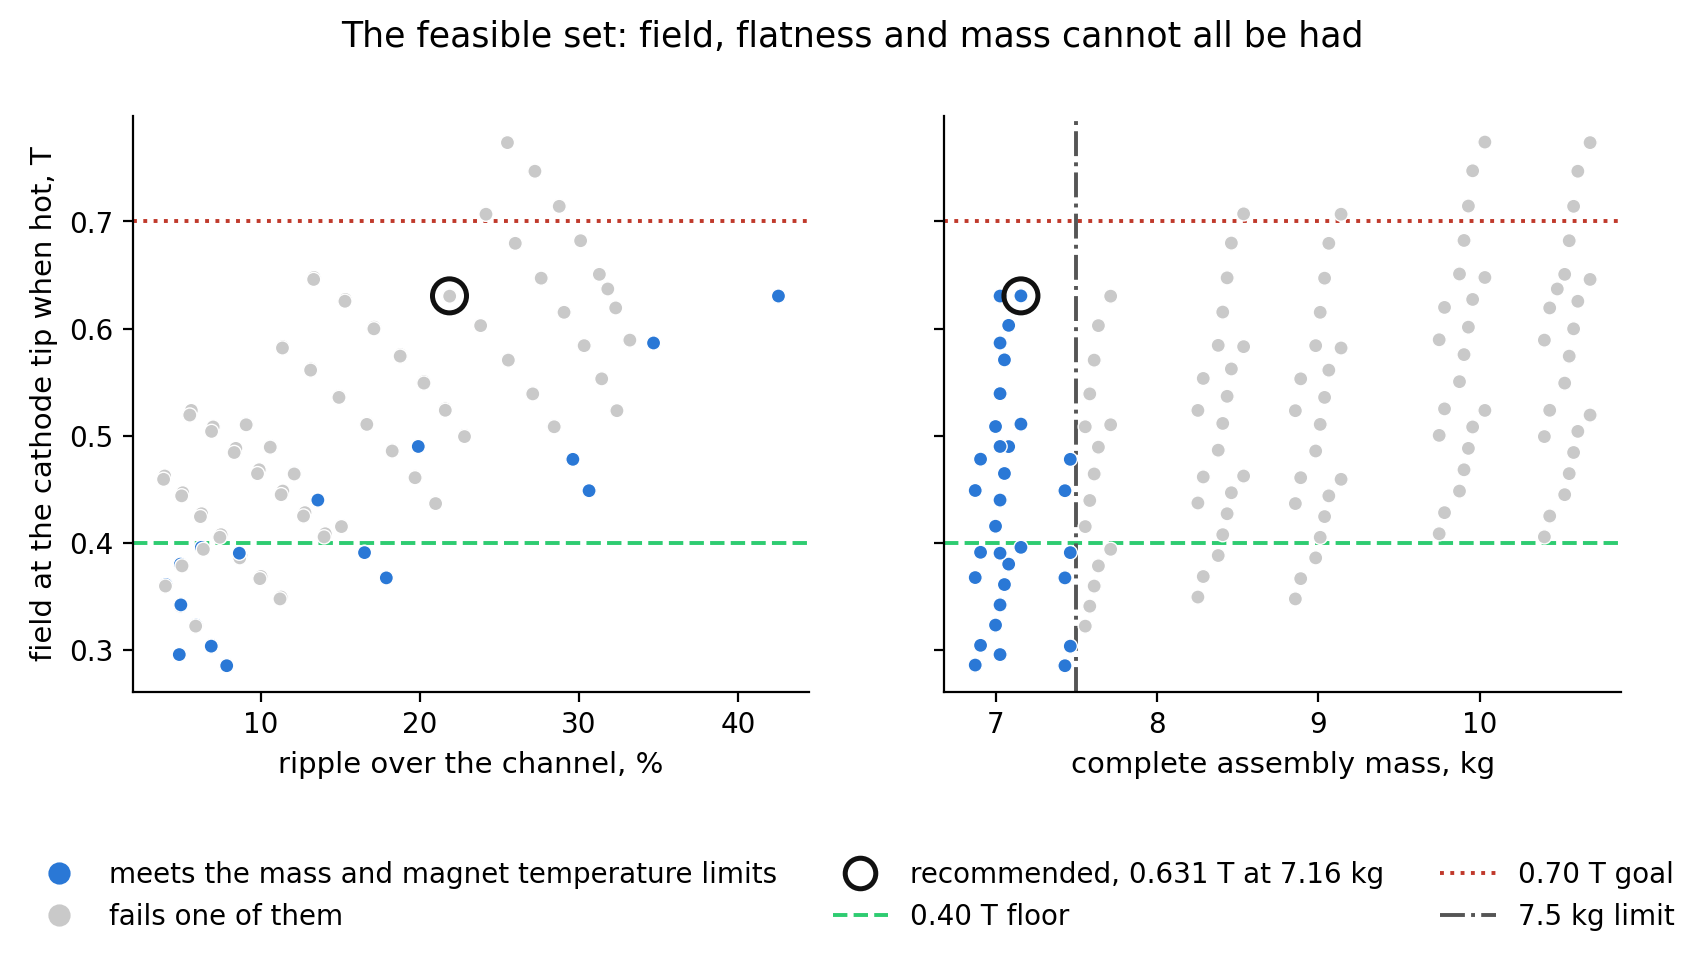
\includegraphics[width=\textwidth]{fig_14_feasible_set.png}
    \caption{Every one of the 136 cold magnetostatic builds, scaled to its own
    solved magnet temperature. The recommended build is circled: it is the
    strongest field available anywhere inside the 7.5~kg mass limit.}
    \label{fig:feasible}
\end{figure}

\textbf{The 0.70~T goal is not reachable inside 7.5~kg, and the magnetics are
not what stops it.} The lightest build in the whole sweep that reaches it gives
0.707~T at 8.54~kg, and it differs from the recommended build in one dimension:
the magnet outside diameter goes from 94 to 104~mm, taking the thruster from
114 to 124~mm across. Every other part is unchanged. So the trade the customer
faces is 0.63~T at 7.17~kg against 0.71~T at 8.54~kg, and it is a mass
decision, not a magnetics one.

% =====================================================================
\section{The One Decision to Settle Before the Magnets Are Ordered}
\label{sec:decision}
% =====================================================================

The recommended build meets the field floor with margin, meets the magnet
temperature target with margin, and meets the mass limit. It does not meet the
field \emph{shape} requirement, and that is worth putting plainly rather than
burying.

End cap thickness is the cheapest lever in the whole design and also the most
expensive one. Thicker caps push more flux across the bore, which is where the
field comes from, but they also concentrate it near the ends, so the profile
stops being uniform. Table~\ref{tab:caps} is that trade at constant mass, in
the same envelope, with every other part identical.

\begin{table}[H]
\centering
\caption{End cap thickness, with the radial build and the envelope held fixed.
Only the tile schedule changes between these three. ``Uniform length'' is how
many millimetres of axis are held within 10\% of the peak field.}
\label{tab:caps}
\begin{tabular}{lrrrr}
\toprule
\textbf{End caps} & \textbf{Cold field} & \textbf{Hot field} &
\textbf{Uniform length} & \textbf{Mass} \\
\midrule
8~mm  & 0.420~T & 0.396~T & 48.0~mm & 7.16~kg \\
\textbf{12~mm} & \textbf{0.542~T} & \textbf{0.511~T} & \textbf{40.8~mm} & \textbf{7.16~kg} \\
16~mm, as recommended & 0.669~T & 0.631~T & 31.5~mm & 7.16~kg \\
\bottomrule
\end{tabular}
\end{table}

Read the middle row carefully. \textbf{Twelve millimetre caps meet every
requirement in this note at once}: 0.511~T hot against a 0.40~T floor, 40.8~mm
of uniform field against a 40~mm requirement, the same 72~\degC{} magnets and
the same 7.16~kg. Sixteen millimetre caps buy 23\% more field and give up a
quarter of the uniform length, taking it below the written requirement.

Which is right depends on something only the customer can answer: whether the
40~mm figure is a real requirement or a target inherited from solenoid
practice. The supervisor's own words were that 0.7~T would bring advantages
\emph{provided the field shape is still what is needed}, so the question is
already half asked.

\textbf{It has to be answered before the tiles are made}, because thickness and
magnetisation are both fixed at manufacture and neither can be changed
afterwards. Nothing else in the package moves: the same casing, the same
sleeve, the same rear stack, the same eight-tile rings, the same drawings. Only
the ring heights on AFMPDT3-003 change, from five rings of 16~mm to a rear cap
of 12, four core rings of 14 and a front cap of 12.

% =====================================================================
\section{Limitations}
\label{sec:limits}
% =====================================================================

\begin{enumerate}[itemsep=4pt]
  \item \textbf{The recommended build was not solved in the coupled solver,
        and the reason is an ordering defect in the study rather than a
        judgement.} The coupled script runs before the down-selection and its
        case list was written in advance, one or two parameters at a time off
        the baseline, to answer specific questions: which rear concept, how
        good the sink has to be, what thicker caps buy, what a larger envelope
        buys. The down-selection then picked a build that changes three of
        those at once, a 2~mm wall with a 1~mm break and 16~mm caps, and that
        combination is not in the list. The nearest coupled case has the 16~mm
        caps on the baseline wall and break. The summary script guards against
        the coupled results being missing altogether but not against the
        selected build being absent from them, so nothing flagged it.

        What this costs is smaller than it sounds. Both inputs are solved
        exactly for this geometry: the field by the magnetostatic sweep and the
        temperatures by the thermal sweep. What is missing is letting the
        remanence read the local temperature point by point instead of applying
        one scale factor, and Section~\ref{sec:verif} measures that difference
        across thirteen coupled cases and finds it conservative by up to 1.4\%.
        \textbf{The fix is one more coupled case and about thirty minutes of
        solver time}, and it should be run before the magnets are ordered.
  \item \textbf{Four figures are drawn for the nearest exported build rather
        than for the recommended one}, and each says so on its own face. Full
        spatial maps were exported for a handful of builds because they are
        large; every scalar quantity in this note is for the recommended build.
        Nothing quantitative rests on those four figures.
  \item \textbf{The discharge model is a uniform conductor} at a median Hall
        parameter of 235, where the real conductivity is a tensor. Read the current paths
        as shape, not as exact values.
  \item \textbf{The cathode is absent from the thermal model}, which makes the
        reported temperatures slightly optimistic.
  \item \textbf{Propellant injection manifold design.} Six 0.9~mm injection
        orifices distributed on a 16~mm pitch circle maintain the plenum pressure
        between 7.6 and 25.4~Torr across a 9 to 30~mg/s argon flow rate, ensuring
        stable operation on the high-pressure branch of the Paschen curve. The
        external propellant connection and cathode feedthrough both interface at
        the rear, requiring planar co-integration with the external cold plate
        assembly.
  \item \textbf{Vacuum facility pumping speed is still unknown.} It sets the
        testable flow rate and therefore which part of the operating map can
        actually be demonstrated.
  \item \textbf{Nothing above 130~\degC{} should be quoted for demagnetisation},
        for the reason given in Section~\ref{sec:field}.
\end{enumerate}

% =====================================================================
\section{Drawings}
\label{sec:drawings}
% =====================================================================

Ten sheets follow, at A3. They are produced by
\texttt{scripts/report\_drawings.py} from the same dimensions the analysis uses
and the same file the parts list in Table~\ref{tab:bom} is computed from, so a
dimension cannot move in one place and not the other.

\begin{table}[H]
\centering
\caption{Drawing index.}
\label{tab:drawings}
\begin{tabular}{ll}
\toprule
\textbf{Sheet} & \textbf{Content} \\
\midrule
AFMPDT3-001 & General arrangement and bill of materials \\
AFMPDT3-002 & Anode barrel \\
AFMPDT3-003 & Magnet tiles and the magnetisation schedule \\
AFMPDT3-004 & Iron return casing \\
AFMPDT3-005 & Standoff sleeve and radiation shield \\
AFMPDT3-006 & Mounting plate: hand-off boss and magnet shelf \\
AFMPDT3-007 & Spreader \\
AFMPDT3-008 & Isolation plate \\
AFMPDT3-009 & Front retaining ring \\
AFMPDT3-010 & Cathode rod and insulating bush \\
\bottomrule
\end{tabular}
\end{table}

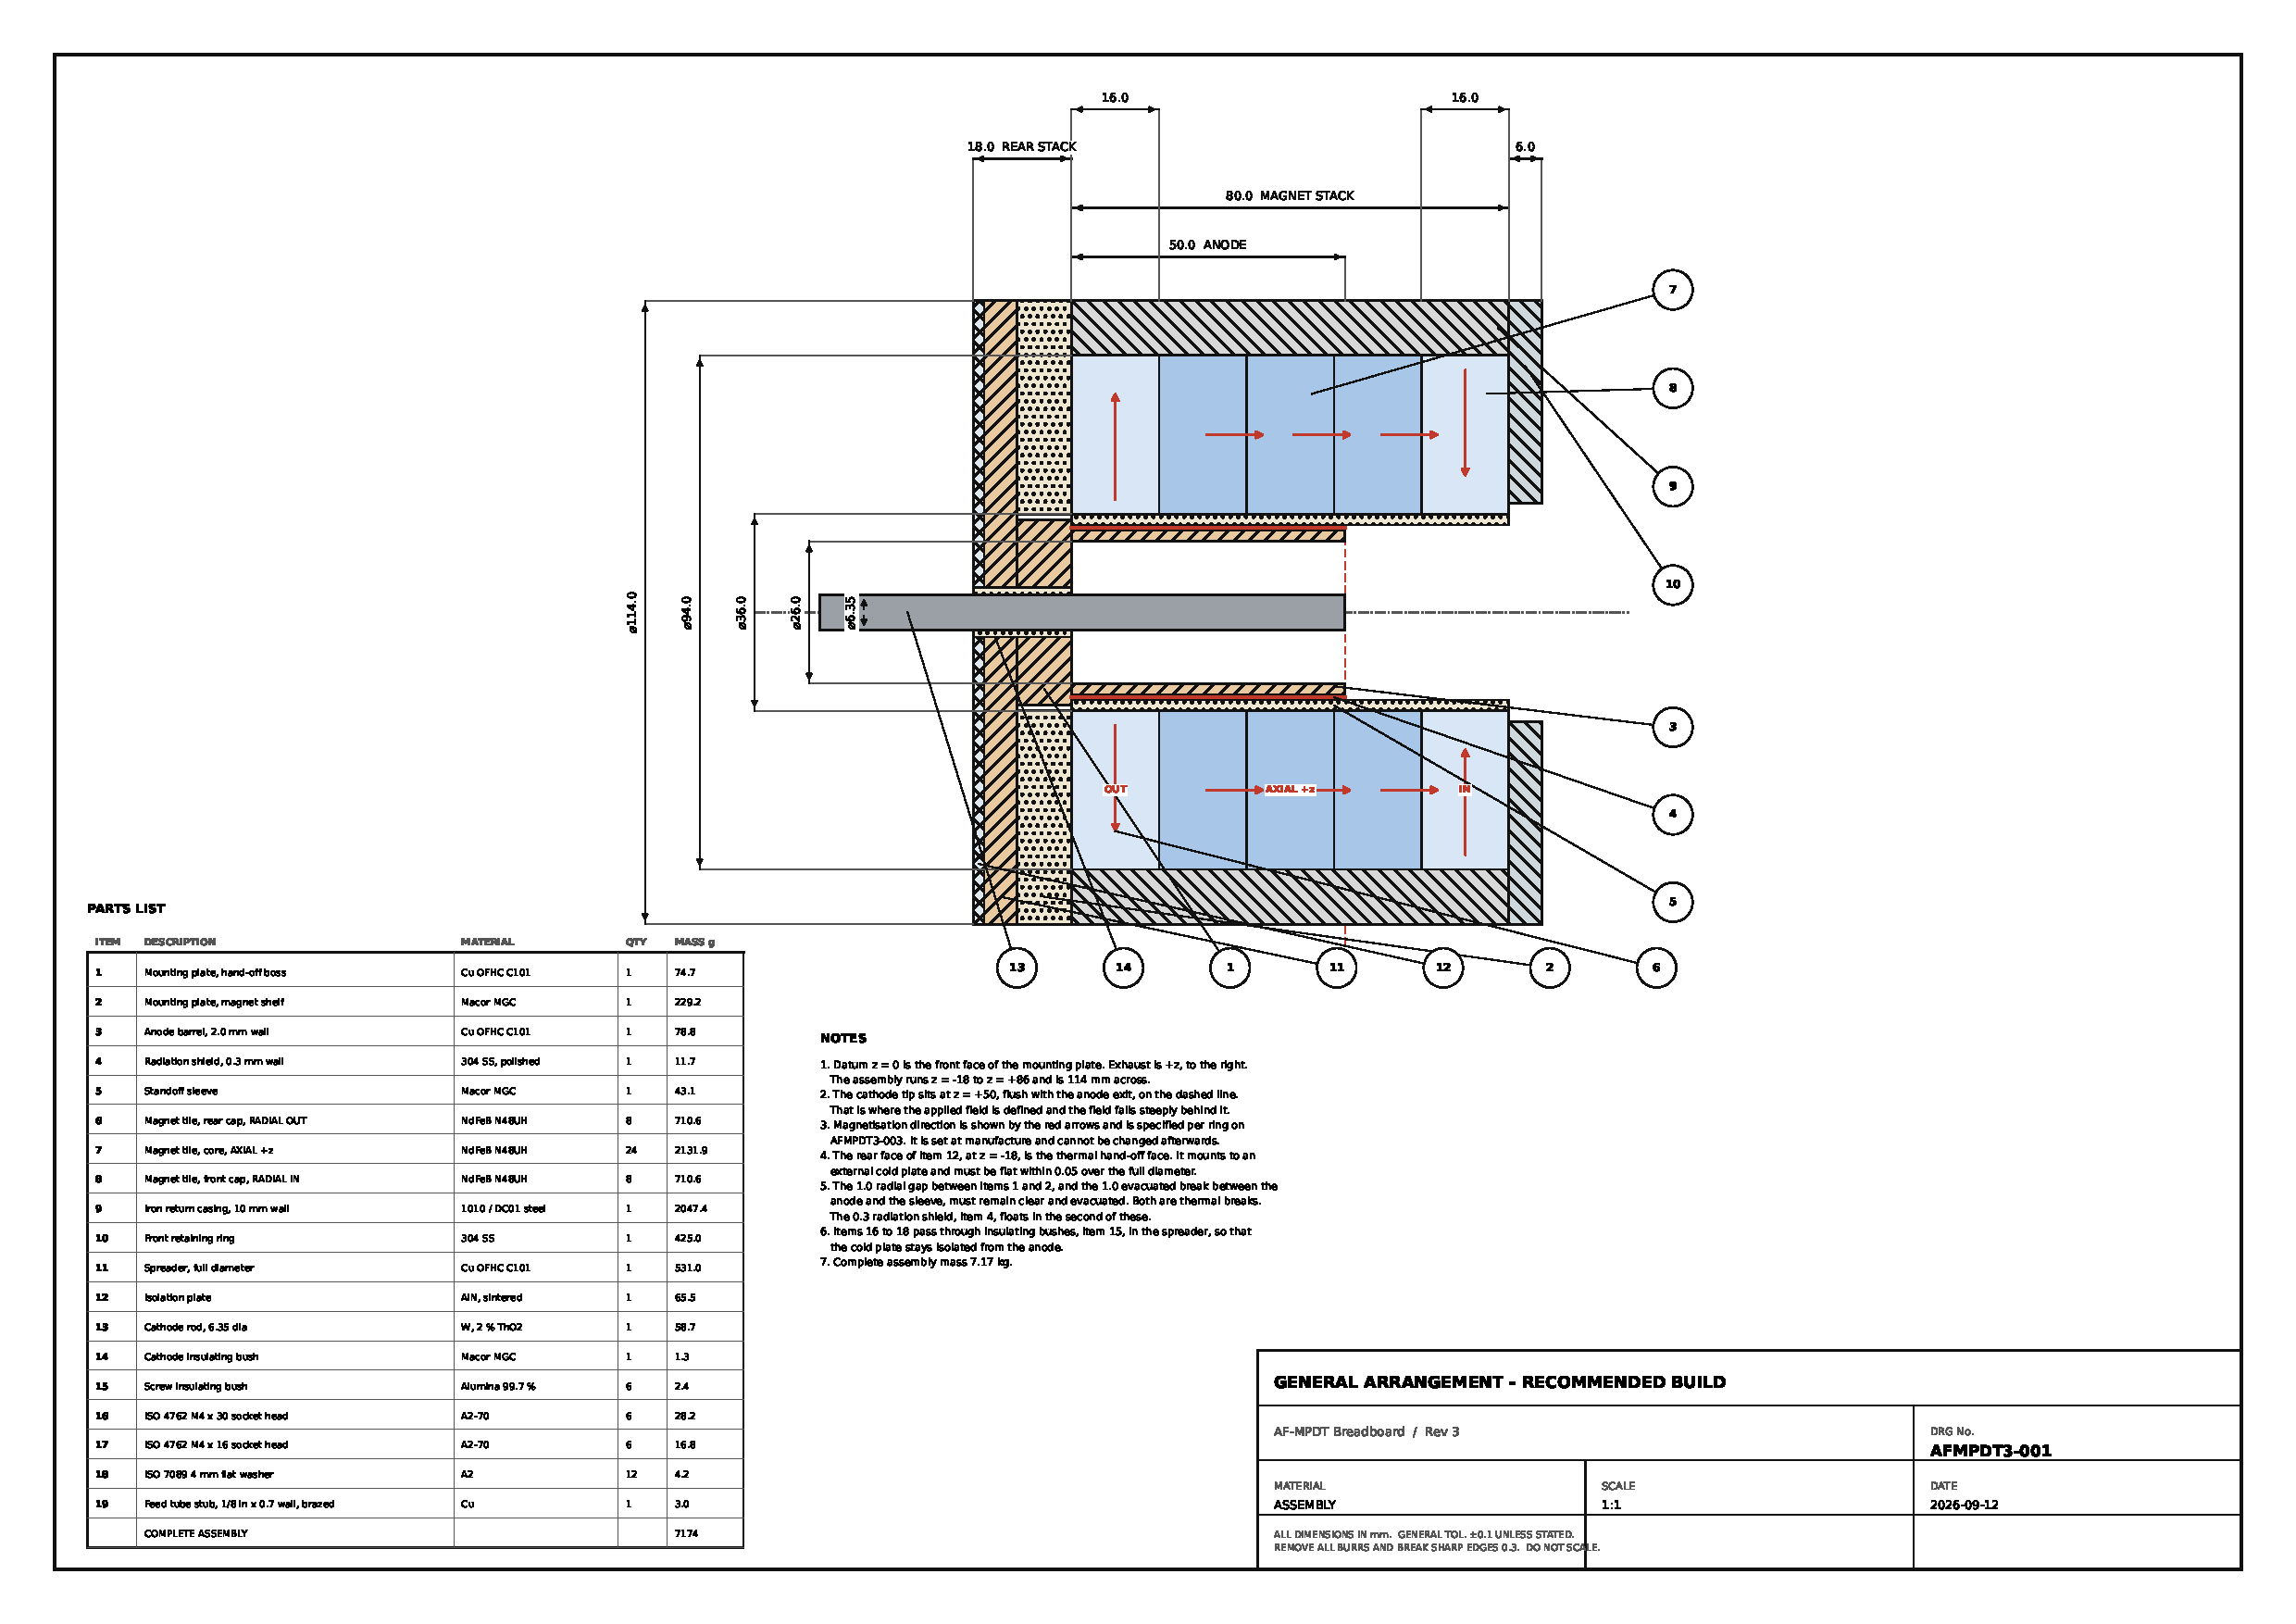
\includepdf[pages=-,fitpaper=true]{drawings/AFMPDT_Rev3_drawing_set.pdf}

\end{document}
